\documentclass[a4paper]{article}

% Hungarian language
% The provided magyar.ldf and huhyphn.tex files are used
% The locations on my system:
% /usr/share/texmf-dist/tex/generic/babel-hungarian/magyar.ldf
% and
% /usr/share/texmf-dist/tex/generic/hyphen/huhyphn.tex
\PassOptionsToPackage{defaults=hu-min}{magyar.ldf}
\usepackage[magyar]{babel}

% Used to remove numbering from sections
\usepackage{titlesec}

% For figures
\usepackage{graphicx}
% For subfigures
\usepackage{subcaption}

% xcolor package for minted and hyperref
\usepackage{xcolor}
% Light gray background for code snippets
\definecolor{codebg}{RGB}{240, 240, 240}
\usepackage[colorlinks=true, linkcolor=black, filecolor=black, urlcolor=blue]{hyperref}

% Used to render code snippets
\usepackage{minted}
% For \FloatBarrier
\usepackage{placeins}

% No numbering for sections (eg. Első Hét)
\titleformat{\section}{\Large\bfseries}{}{0pt}{}{}

% Inline code snippets
\newcommand{\inlts}[1]{\mintinline[breaklines, breakanywhere]{typescript}{#1}}
\newcommand{\inltxt}[1]{\mintinline[breaklines, breakanywhere]{text}{#1}}

\title{Szakmai Gyakorlat Munkanapló}
\author{Bauer Brúnó Csaba}
\date{2024. 12. 30.}

\begin{document}

% Title Page
\maketitle
\thispagestyle{empty}
\newpage

% Table of Contents
\clearpage
\tableofcontents
\newpage
\phantomsection

\section{Első Hét}

\subsection{Első nap, projektfeladat ismertetése (09.04.)}

Az első nap munkavédelmi, tűzvédelmi, és egyéb céges oktatásokon, valamint cégbemutatón vettem
részt. Ez után következett a projektfeladatom ismertetése

\subsubsection*{Projektfeladat}

A két hónapos időszak alatt egy webalkalmazást kell fejlesztenem a cég számára. A fő cél az, hogy egy
olyan felületet hozzak létre, ahol az alkalmazottak nyomon követhetik a munkaidejüket, ugyanakkor
fontos, hogy lehetőség legyen a későbbi bővítésekre is. További követelmény, hogy az autentikáció és
a felhasználói adatok lekérdezése a cégen belül hamarosan bevezetésre kerülő Active Directory
címtárszolgáltatás integrációjával történjen. A dolgozók beléptetése az EntraPass Special Edition
szoftvercsomag segítségével történik, így ez lesz a forrása a beléptetési adatoknak.

\subsection{Active Directory, tech stack, szerver telepítés, tervezés megkezdése (09.05.)}

Mivel az Active Directory, illetve az LDAP protokoll számomra ismeretlen technológiák, ezért először
ezekkel kezdtem el ismerkedni. (Fontosabb források:
\href{http://web.archive.org/web/20240315064825/http://ldapjs.org/guide.html}{LDAP.js Guide (Web Archive)}
\href{https://en.wikipedia.org/wiki/Lightweight_Directory_Access_Protocol}{Lightweight Directory Access Protocol (Wikipedia)})\\

Később rá is találtam egy JavaScript (TypeScript) könyvtárra \inlts{ldapts} néven
(\href{https://github.com/ldapts/ldapts}{ldapts}), amely könyvtár alkalmas lesz az Active Directory szerverrel
(továbbiakban: AD szerver) való kommunikálásra. Elkezdtem ismerkedni a libraryvel, sikerült vele az
AD szerverhez kéréseket küldeni. A könyvtár – a webalkalmazás szempontjából - két legfontosabb
függvénye:

\FloatBarrier
\begin{minted}[bgcolor=codebg, breaklines, breakanywhere, fontsize=\small]{typescript}
bind(dnOrSaslMechanism, [password], [controls])
\end{minted}

A \inlts{bind} függvény egy bind operációt kezdeményez az AD szerver felé. Ezzel az operációval
autentikálhatjuk magunkat az AD szerver felé. Sikeres bind után, az azt követő kérések már az adott
felhasználó nevével történnek.

\FloatBarrier
\begin{minted}[bgcolor=codebg, breaklines, breakanywhere, fontsize=\small]{typescript}
search(baseDN, options, [controls])
\end{minted}

A search operációval LDAP entrykre - pl. felhasználókra - kereshetünk. A kereséshez LDAP filtert kell
írni. Mivel ezek a filterek - hasonlóan az SQL lekérdezésekhez - sérülékenyek injection támadásra, ezért
escape-elni kell majd őket.

\subsubsection*{Tech Stack}
Technológiák terén annyi megkötés volt, hogy lehetőleg olyan eszközökkel dolgozzak, amelyeket az
egyetemen is megismerhettünk. Mivel a Web programozás 2 tantárgy keretében lehetőség nyílik a
SvelteKit keretrendszerrel/meta frameworkkel való megismerkedésre, illetve nekem is a JavaScript
alapú webfejlesztésben van a legnagyobb tapasztalatom, így erre esett a választásom.\\

Backend/Frontend:
\begin{itemize}
  \item Nyelv: TypeScript
  \item Keretrendszer: SvelteKit
  \item CSS: Tailwind, Skeleton – UI Toolkit for Svelte and Tailwind
  \item ORM: drizzle ORM
\end{itemize}

Adatbázis:
\begin{itemize}
  \item PostgreSQL
\end{itemize}

\subsubsection*{Szerver telepítés}
A szerverhez biztosított a cég két 500 GB-os HDD-t, melyeket elsősorban beszereltem. A webszerverre
Debian 12 disztribúciót telepítettem a stabilitása miatt. Telepítés során a két HDD-t szoftveres RAID1-
be konfiguráltam. A RAID1 miatt ugyan lassabb lesz az írás a merevlemezre, valamint az 1 TB helyett
mindössze 500GB lesz elérhető, azonban a tükrözés miatt nagyobb lesz a hibatűrés.

\subsubsection*{Tervezés megkezése}
Ezek után a projekt megkezdéséhez szükséges, kezdetleges terveket készítettem el.
(Lásd \aref{fig:login_diagram}. és \aref{fig:further_requests_diagram}.~ábrákat)\\

\begin{figure}[ht]
  \centering
  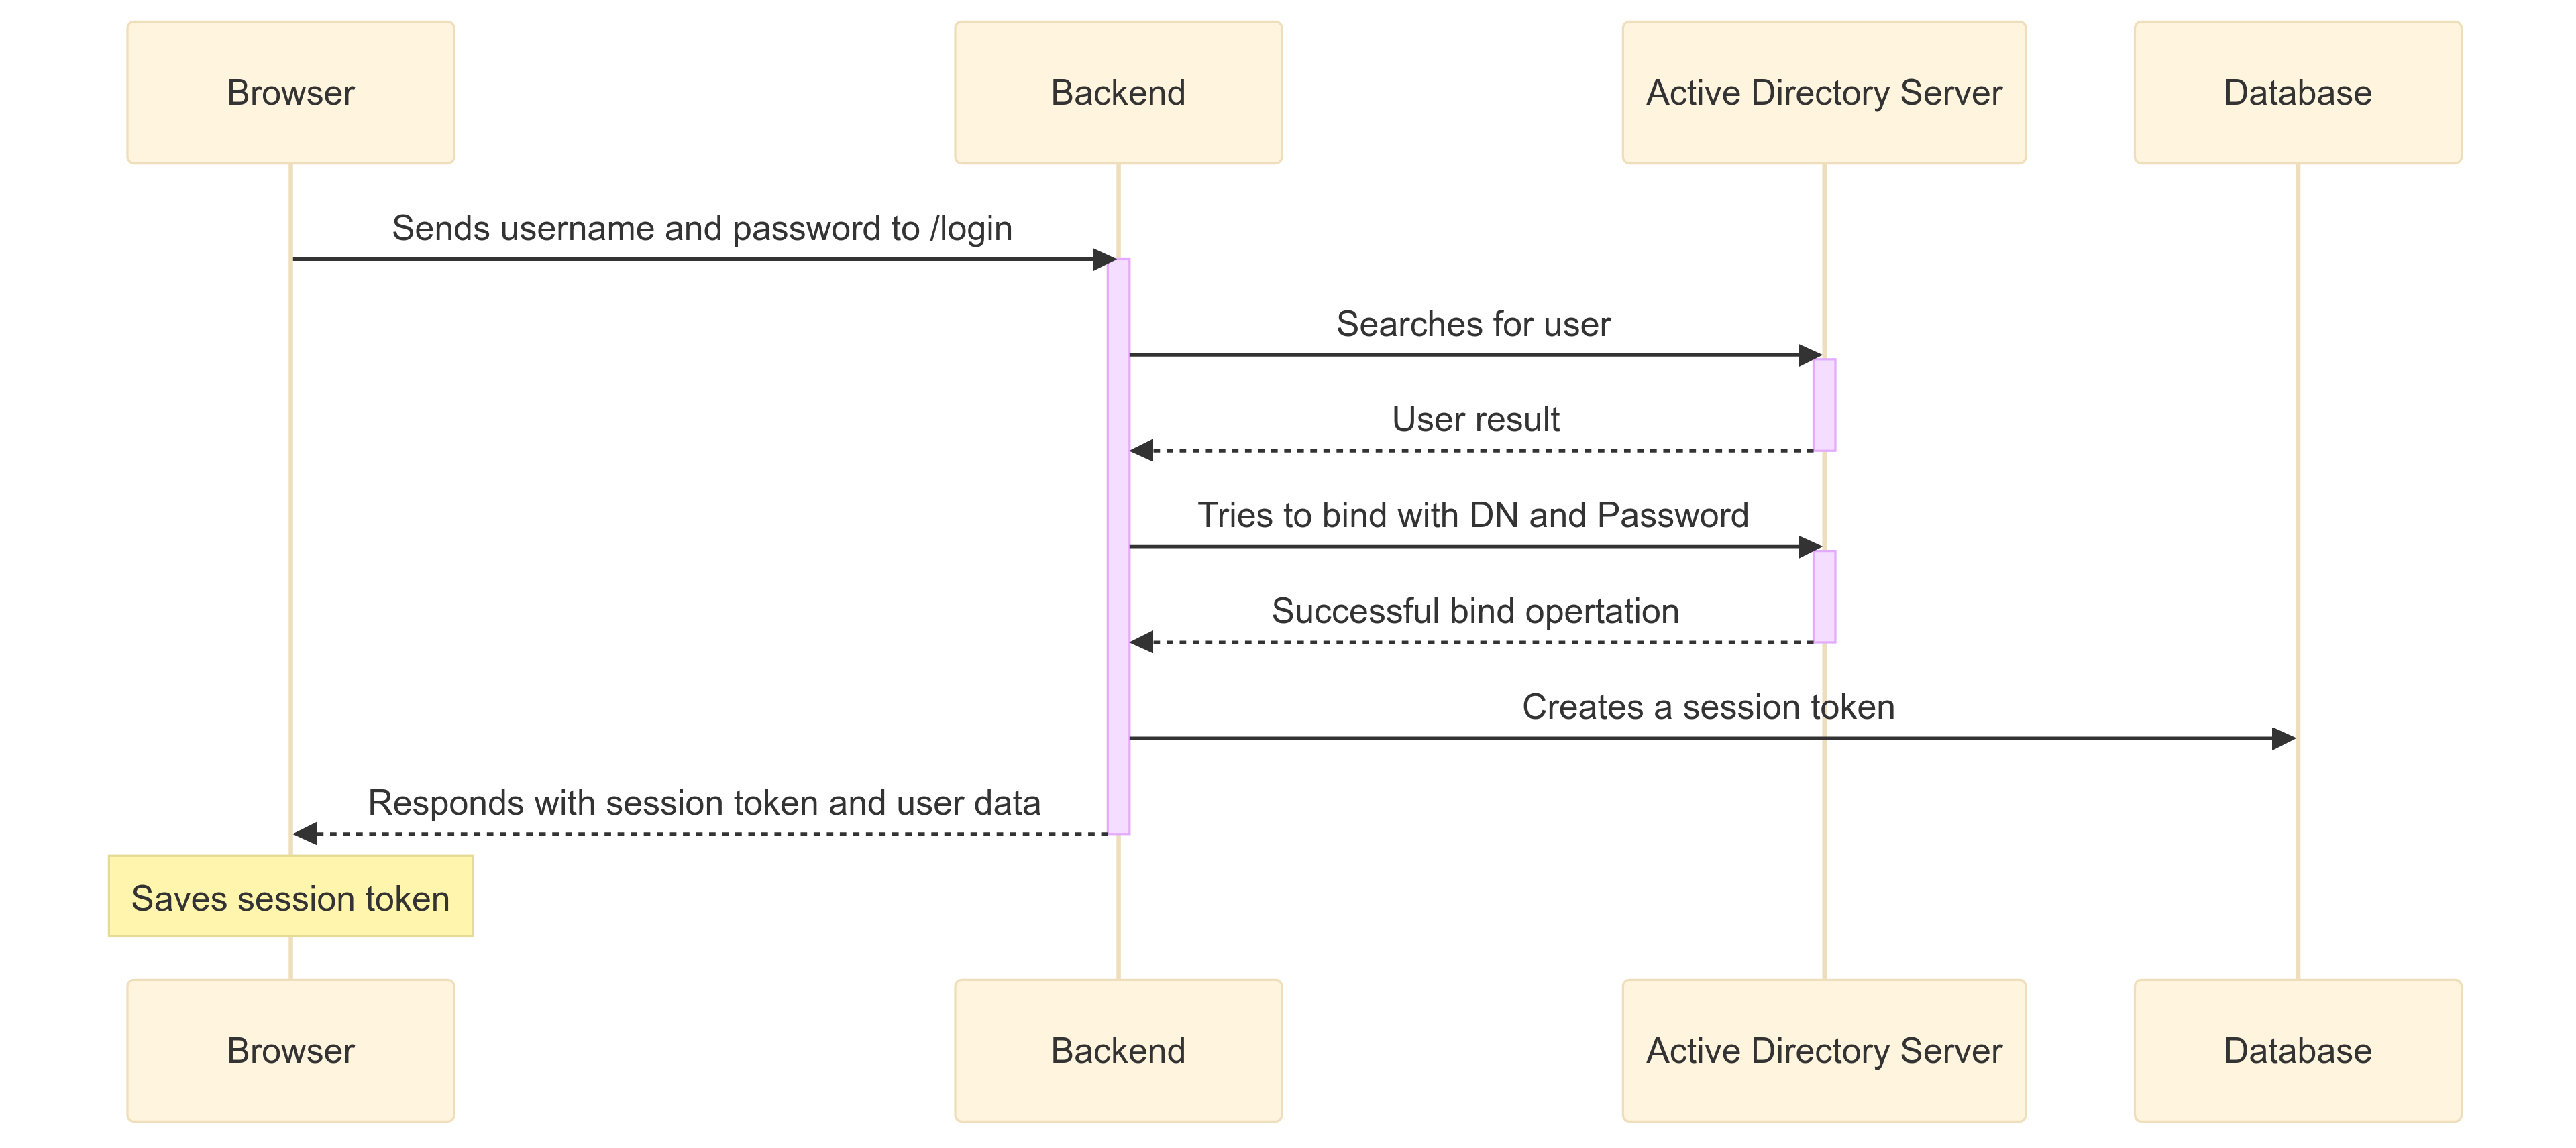
\includegraphics[width = 0.8\textwidth]{images/login_diagram.png}
  \caption{Bejelentkezés}
  \label{fig:login_diagram}
\end{figure}
\begin{center}
\end{center}

\begin{figure}[ht]
  \centering
  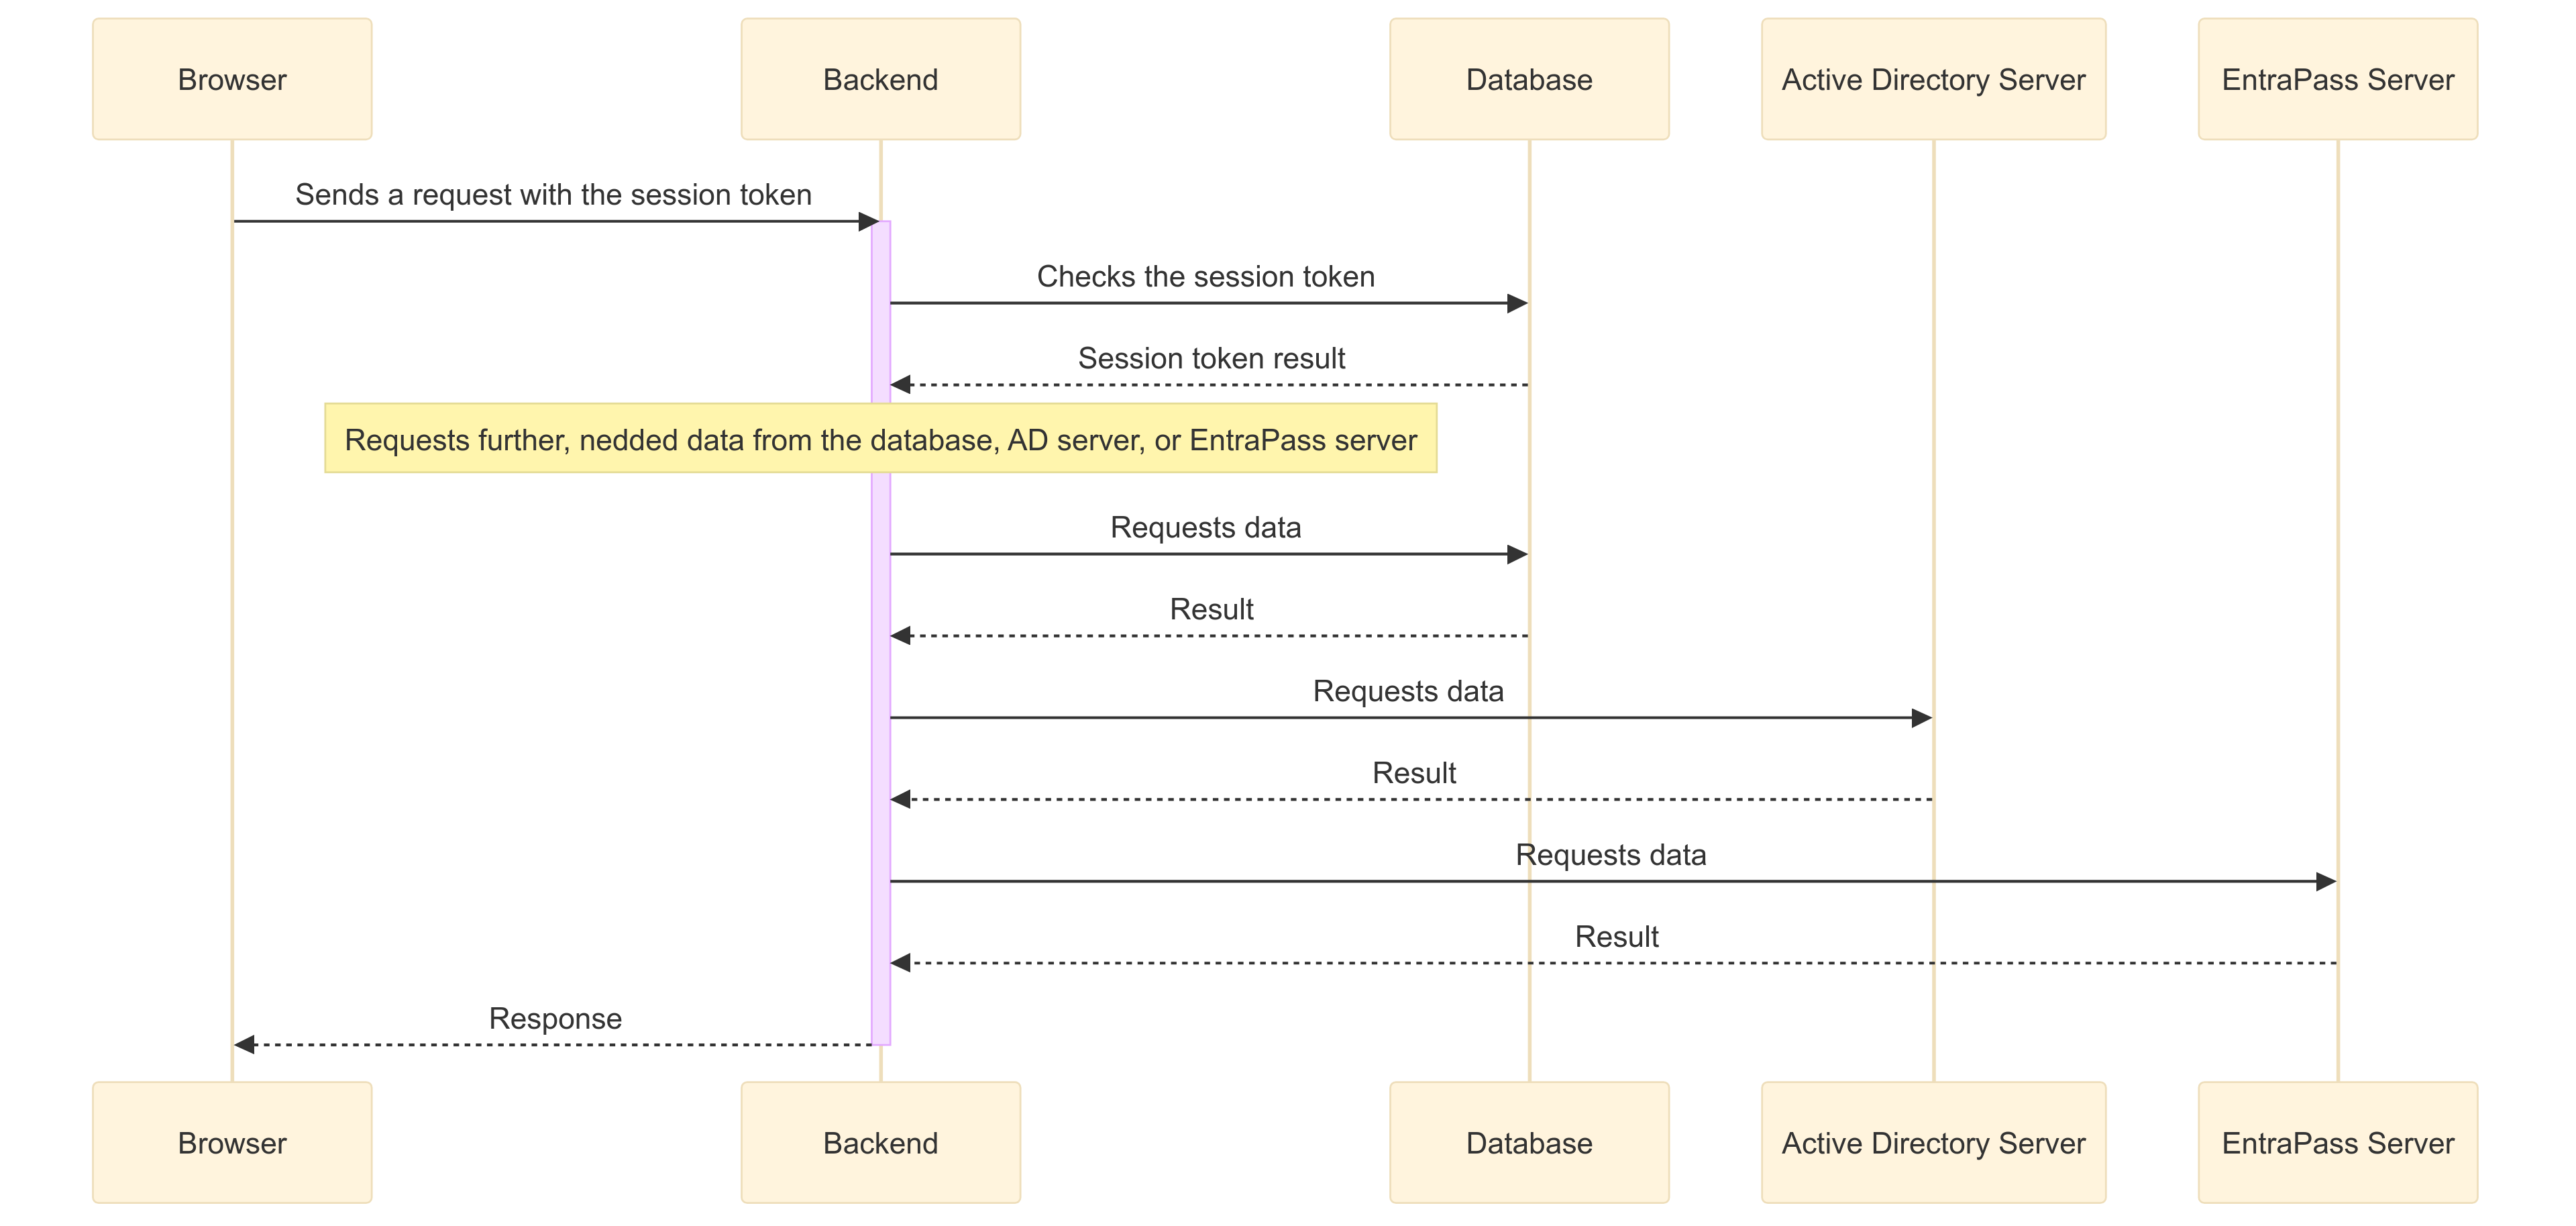
\includegraphics[width = 0.8\textwidth]{images/further_requests_diagram.png}
  \caption{További kérések}
  \label{fig:further_requests_diagram}
\end{figure}
\begin{center}
\end{center}

\subsection{SvelteKit projekt elkezdése (09.06.)}

A mai nap a projekt elkezdésével telt. Létrehoztam a SvelteKit projektet, telepítettem, illetve
beállítottam a Skeleton UI toolkitet, amely UI komponenseket biztosít a gyorsabb fejlesztés
érdekében. Biome.js-t is telepítettem, amely egy fejlesztői eszköztár kód formázásra és ellenőrzésre
(linting).\\

Bár az i18n (több nyelv támogatása) nem volt a projekt követelményeiben, mégis úgy döntöttem, hogy
már az elején implementálom, hogy később – amennyiben szükség lesz rá - egyszerűbb legyen bővíteni
a nyelvi beállításokat.\\

A felhasználói élmény növelése érdekében implementáltam a világos/sötét mód támogatást, így a
felhasználók váltogathatnak a témák között. Végül létrehoztam az alkalmazás alapvető felépítését:
tartalmaz egy fejlécet, egy fő tartalmi részt (body), és egy láblécet. (\ref{fig:dark_light_modes}.~ábra)\\

\begin{figure}[ht]
    \centering
    \begin{subfigure}[b]{0.45\textwidth}
        \centering
        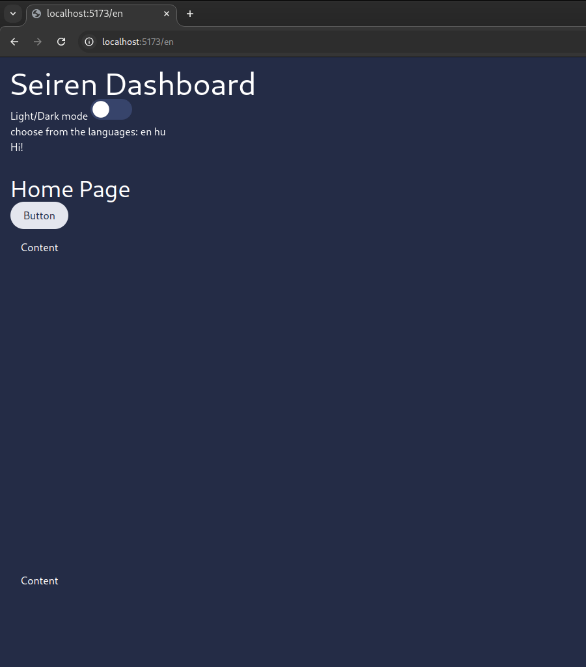
\includegraphics[width=\textwidth]{images/dark_preview.png}
        \caption{Sötét mód, angol nyelv}
        \label{fig:dark_mode}
    \end{subfigure}
    \hfill
    \begin{subfigure}[b]{0.45\textwidth}
        \centering
        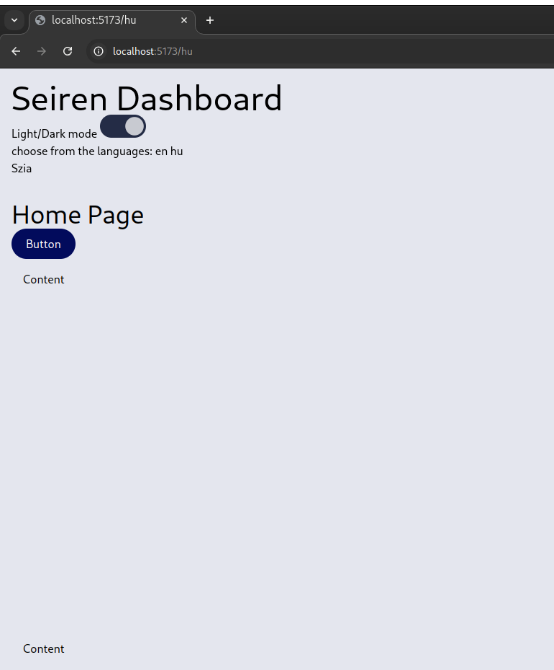
\includegraphics[clip, trim = 0 24 0 0, width=\textwidth]{images/light_preview.png}
        \caption{Világos mód, magyar nyelv}
        \label{fig:light_mode}
    \end{subfigure}
    \caption{Sötét és világos mód}
    \label{fig:dark_light_modes}
\end{figure}

\subsection{Active Directory VM, kód futtatása az alkalmazás indulásakor (09.07.)}

Szükség volt egy dedikált Active Directory szerverre, hogy ne az éles szervert kelljen használnom a
fejlesztéshez. Először egy Docker konténerre gondoltam, azonban mint kiderült, nincsen egy az
eredetihez még csak hasonló megoldás sem, lévén az Active Directory egy Windows technológia. A
megoldás egy Windows Server VM lett, aminek a telepítését dokumentáltam. Az Active Directory
telepítéséhez nagy segítség volt ez a YouTube videó: \href{https://youtu.be/MHsI8hJmggI?si=t0c5f8Z-
2RUdvrnV}{ How to Setup a Basic Home Lab Running Active Directory (Oracle VirtualBox) | Add Users w/PowerShell (YouTube)}.

\subsubsection*{Kód futtatása az alkalmazás indulásakor}
Mivel a SvelteKit dokumentációjában nem találtam arra módszert, hogy hogyan kell futtatni kódot az
alkalmazás indulásakor, így az interneten keresgéltem. Több módszert is találtam és ki is próbáltam. A
végén arra a megoldásra esett a választásom, hogy a \inlts{hooks.server.ts} fájlba írom azt a kódot, amit
induláskor futtatni kell. Egyetlen hátulütője ennek a megoldásnak az az, hogy dev módban (fejlesztés
közben), nem történik meg automatikusan a kód futtatása, csak az első kérés beérkezése során. Erre
az lett a megoldásom, hogy írtam egy bash szkriptet, ami a dev script indulásával együtt lefut és \inltxt{curl}-
el kéréseket küld a szervernek addig, ameddig az nem válaszol.

\subsection{Active Directory service, logolás (09.08.)}

Az Active Directory service-t kezdem el írni, vagyis azt a fájlt, amiben az AD szerverrel való
kommunikációhoz szükséges függvények találhatók. Első körben egy \inlts{start} és egy \inlts{stop} függvényt
implementáltam.

\FloatBarrier
\begin{minted}[bgcolor=codebg, breaklines, breakanywhere, fontsize=\small]{typescript}
// lib/services/activeDirectoryService.ts
let ldapClient: LdapClient;
let reconnecting = false;

async function start(activeDirectoryConfig: LdapConfig) { ... }
async function startReconnecting() { ... }
async function stop() { ... }

const activeDirectoryService: ActiveDirectoryService = {
    start,
    stop,
};

export default activeDirectoryService;
\end{minted}

A \inlts{start} függvény lényegében egy LDAP klienst inicializál, majd pedig egy bind operációt hajt végre az
AD szerveren, az alkalmazás számára létrehozott admin felhasználó DN és jelszó párosával.\\

A különböző konfigurációk betöltéséért- mint például az AD szerver hosztja, vagy az előbb említett
admin DN és jelszó – külön modulok felelnek a \inlts{lib/configs} mappában. Ezek a modulok a környezeti
változókat olvassák be az alkalmazás indulásakor (\inlts{hooks.server.ts}) \\

Fontosnak tartom, hogy az alkalmazás a lehető legjobban hibatűrő legyen, ezért azt is implementáltam
a start függvénybe, hogy ha nem sikerül csatlakozni az AD szerverhez, akkor az alkalmazás
próbálkozzon újra csatlakozni. Amennyiben ez mégsem sikerül, logolja a hibát. Annak érdekében, hogy
ez a működés a későbbiekben is könnyen használható legyen, írtam egy \inlts{startReconnecting}
függvényt is.

\subsubsection*{Logolás}

Ezt követően a logolással foglalkoztam. A pino libraryt adtam hozzá a projekthez.

\section{Második Hét}

\subsection{Active Directory service, tesztelés előkészítése (09.11.)}

A mai napon, első körben, két új függvényt írtam az AD servicehez. Ezek az \inlts{authenticateUser}, és
a \inlts{getUserBysAMAccountName} függvények. Az \inlts{authenticateUser} függvény egy DN-t, és egy
jelszót vár paraméterként, inicializál egy új LDAP klienst, amellyel egy bind operációval autentikálja a
felhasználót az AD szerver felé. \\

A \inlts{getUserBysAMAccountName} függvény pedig egy felhasználónevet (sAMAccountName) vár
paraméternek és egy search operációval megpróbálja megkeresni az AD szerveren a felhasználót. A
válaszként kapott felhasználó parseolásához a typebox library-t használom:

\FloatBarrier
\begin{minted}[bgcolor=codebg, breaklines, breakanywhere, fontsize=\small]{typescript}
// lib/types/user.ts
import { Type } from "@sinclair/typebox";
import type { Static } from "@sinclair/typebox";

export const activeDirectoryUserSchema = Type.Object({
    employeeID: Type.String(),
    distinguishedName: Type.String(),
    sAMAccountName: Type.String(),
    employeeNumber: Type.String(),
    memberOf: Type.Union([Type.String(), Type.Array(Type.String())], {
        default: "",
    }),
    sn: Type.String(),
    givenName: Type.String(),
    displayName: Type.String(),
    pwdLastSet: Type.String(),
});

export type ActiveDirectoryUser = Static<typeof activeDirectoryUserSchema>;
export const activeDirectoryUserValidator: Validator<ActiveDirectoryUser> =
    createValidator<ActiveDirectoryUser>(activeDirectoryUserSchema);
\end{minted}

Mivel a projekt követelményei közé tartozott az is, hogy az alkalmazás az AD-ben szereplő jelszavak
lejárati dátumait vegye figyelembe a session kezelésnél, így a pwdLastSet attribútumot is át kellett
konvertáljam dátum objektummá, melyet az alábbi függvénnyel oldottam meg:

\FloatBarrier
\begin{minted}[bgcolor=codebg, breaklines, breakanywhere, fontsize=\small]{typescript}
// lib/utils/activeDirectoryUtils.ts
export function parseActiveDirectoryDate(activeDirectoryDate: string): Date {
	const truncatedPwdLastSet = activeDirectoryDate.substring(
		0,
		activeDirectoryDate.length - 4,
	);

	const windowsEpoch = Date.UTC(1601, 0, 1);
	return new Date(windowsEpoch + Number.parseInt(truncatedPwdLastSet));
}
\end{minted}

\subsubsection*{Tesztelés előkészítése}
A tesztelés nem szerepelt a projektkövetelmények között, valamint idő szűkében nem is tudnék 100\%-
os kódlefedettséget elérni. Ennek ellenére az alkalmazás fontosabb részeihez – amennyiben időm
engedi – írok unit teszteket. (Integrációs, illetve e2e teszteket még nem biztos, hogy fogok írni, de ha
szükségét érzem, és időm engedi, akkor azokat is fogok.) \\

Az AD service is egy ilyen fontosabb, illetve kérdéses része az alkalmazásnak. Ahhoz, hogy AD service
unit teszteket tudjak írni szükséges egy ”mock” LDAP klienst létrehozni. Ehhez írtam először egy
\inlts{AbstractLdapClient} osztályt, amit majd extendelni fog az \inlts{LdapClient} és a \inlts{MockLdapClient}
osztály. A \inlts{MockLdapClient} osztályra már nem volt időm a mai nap.

\subsection{MockLdapClient, ActiveDirectoryService osztállyá alakítása, tesztek
írása (09.12.)}

\subsubsection*{MockLdapClient}

A mai napot a \inlts{MockLdapClient} osztály implementálásával kezdtem. Egyelőre csak két függvényt –
\inlts{search} és \inlts{bind} – kellett megírnom, melyek a \inlts{tests/mocks/data/} mappában találhatók alapján
futnak le, illetve dobnak hibákat.

\subsubsection*{ActiveDirectoryService osztállyá alakítása}

Annak érdekében, hogy az AD service-t megfelelően lehessen tesztelni, (”singleton”) osztállyá
alakítottam át azt, így minden tesztet külön példánnyal lehet végrehajtani.

\FloatBarrier
\begin{minted}[bgcolor=codebg, breaklines, breakanywhere, fontsize=\small]{typescript}
// lib/services/ActiveDirectoryService.ts
class ActiveDirectoryService {
    protected static _instance: ActiveDirectoryService | undefined = undefined;
    static initialize(
        ldapClient: AbstractLdapClient,
        activeDirectoryConfig: ActiveDirectoryConfig,
    ) {
        if (!ActiveDirectoryService._instance) {
            ActiveDirectoryService._instance = new ActiveDirectoryService(
                ldapClient,
                activeDirectoryConfig,
            );
        }
        return ActiveDirectoryService._instance;
    }

    static get instance(): ActiveDirectoryService {
        if (!ActiveDirectoryService._instance) {
            throw new Error(...);
        }
        return ActiveDirectoryService._instance;
    }

    private ldapClient: AbstractLdapClient;

    ...

    protected constructor(
        ldapClient: AbstractLdapClient,
        activeDirectoryConfig: ActiveDirectoryConfig,
    ) {
        this.ldapClient = ldapClient;
        this.activeDirectoryConfig = activeDirectoryConfig;
    }

    async start() { ... }
    async authenticateUser(bindDN: string, password: string): Promise<boolean> { ... }
    async getUserBysAMAccountName(sAMAccountName: string): Promise<User> { ... }
    ...
}
\end{minted}

\subsubsection*{Tesztek írása}

Ezt követően a következő AD service unit teszteket írtam meg:

\FloatBarrier
\begin{minted}[bgcolor=codebg, breaklines, breakanywhere, fontsize=\small]{text}
// pnpm run test:unit
src/lib/services/ActiveDirectoryService.test.ts (20)
    ActiveDirectoryService Singleton Tests (2)
        should initialize and return the same instance
        should reset the singleton between tests
    start() (5)
        should succeed with correct admin dn and password
        should succeed if service can reconnect after a connection error
        should throw LdapConnectionError if a connection error occures
        should throw UnknownLdapError if an unknown error occures
        should throw LdapAuthenticationError with incorrect admin credentials
    getUserBysAMAccountName() (9)
        should succeed with correct sAMAccountName
        should succeed if user is in multiple groups
        should return user with isAdmin set to true, if user is a member of the
            Admins group
        should throw UserNotFoundError if the user does not exist
        should throw MultipleUsersFoundError when multiple users are found
        should throw an InternalError if one or more active directory attributes are
            missing/incorrect
        should throw an InternalError if the ActiveDirectoryUser cannot be converted
            to a User
        should throw an InternalError if an unknown error occures
        should throw an InternalError if a connection error occures
    authenticateUser (4)
        should return true with correct credentials
        should return false with incorrect credentials
        should throw an InternalError if a connection error occures
        should throw an InternalError if an unknown error occures

\end{minted}

\subsection{Header komponens, Login oldal (frontend) (09.13.)}

A Header komponenst implementáltam először (\ref{fig:header_component}.~ábra). Sikerült teljesen
reszponzívra megírni (\ref{fig:header_component_mobile}.~ábra). Tartalmaz
két – egyelőre placeholder – menüsort, melyekre kattintva egy-egy ”dropdown” jelenik meg, a jobb
sarokban egy ”profil gombot”, melyre kattintva szintén egy dropdown jelenik meg, ahol többek között
ki lehet választani a nyelvet (magyar, angol), illetve változtatni lehet a témán (sötét/világos). Ezen
kívül, a Header bal sarkában egy ”hamburger”, vagyis menü ikon jelenik meg mobileszközökön. Erre
kattintva egy oldalsó menüsor (”drawer”) jelenik meg a placeholder menüpontokkal.

\begin{figure}[ht]
  \centering
  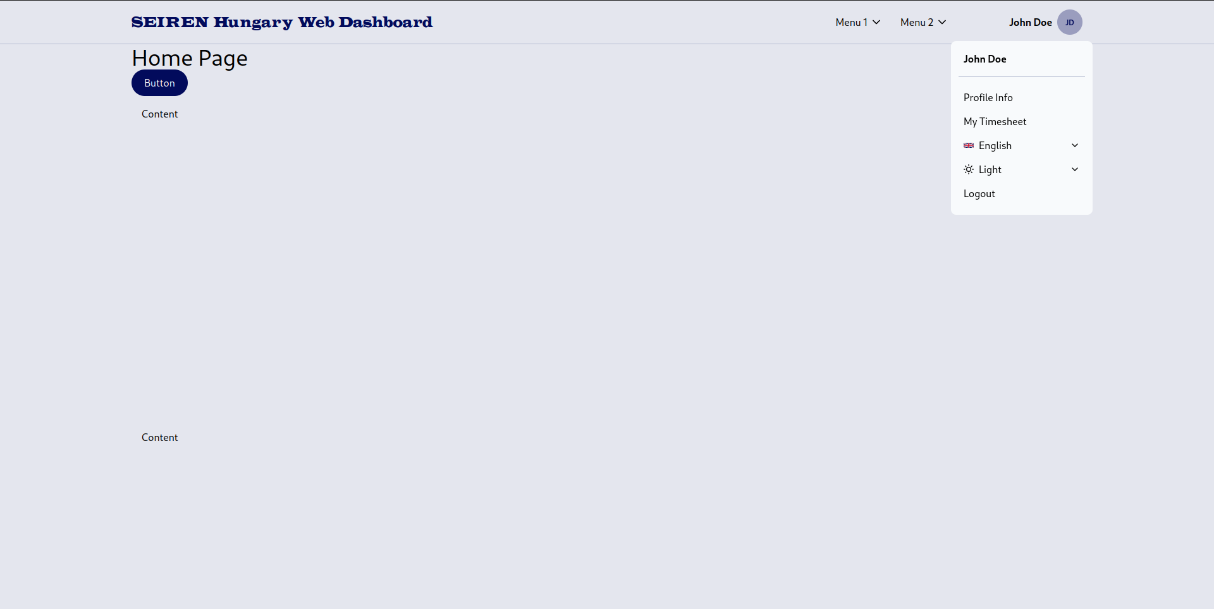
\includegraphics[width = 0.8\textwidth]{images/header.png}
  \caption{Header komponens, asztali méret, világos mód}
  \label{fig:header_component}
\end{figure}
\begin{center}
\end{center}

\begin{figure}[ht]
    \centering
    \begin{subfigure}[b]{0.45\textwidth}
        \centering
        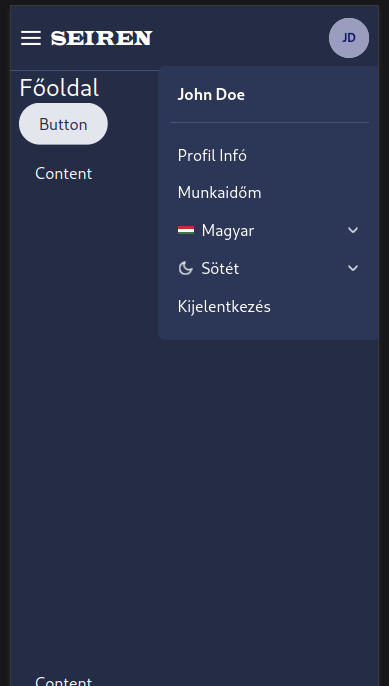
\includegraphics[height=0.4\textheight]{images/header_mobile.png}
        \caption{Mobil méret, sötét mód, magyar nyelv}
        \label{fig:header_mobile_closed}
    \end{subfigure}
    \hfill
    \begin{subfigure}[b]{0.45\textwidth}
        \centering
        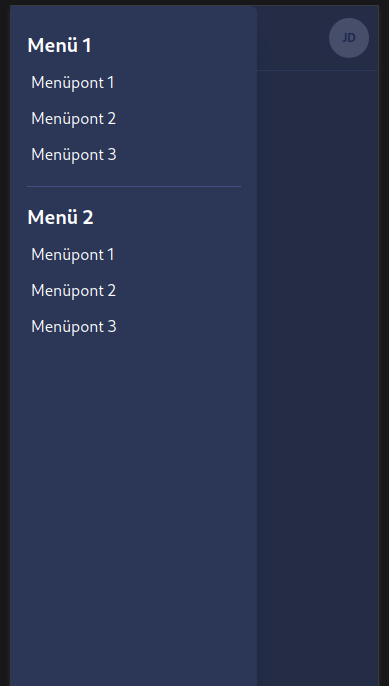
\includegraphics[height=0.4\textheight]{images/header_mobile_open.png}
        \caption{Oldalsó menüsor}
        \label{fig:header_mobile_open}
    \end{subfigure}
    \caption{Header komponens, mobil méret}
    \label{fig:header_component_mobile}
\end{figure}

\subsubsection*{Login oldal (frontend)}
Ezt követően a bejelentkezési oldal frontend részét csináltam meg (\ref{fig:login_page}.~ábra).
A bejelentkezés gomb megnyomásával a böngésző egy \inltxt{POST} kérést küld a szervernek.
Amennyiben sikeres a bejelentkezés, a szerver átirányít a kezdőoldalra, ahol egy
felugró, ”toast” üzenetet jelenít meg az alkalmazás. A toast üzenethez tartozó adatot (szöveg, háttérszín) nem szerettem volna az
URL-en keresztül átadni, ezért azt egy cookie-ban tárolom, melyet a kiolvasás után egyből törlök is.

\begin{figure}[ht]
  \centering
  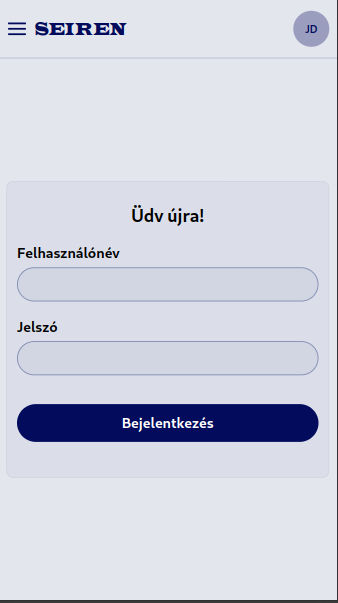
\includegraphics[clip, trim=0 10 1 0, width = 0.3\textwidth]{images/login_page.png}
  \caption{Login oldal, világos mód}
  \label{fig:login_page}
\end{figure}

\subsection{Login backend, session validáció (09.14.)}

A bejelentkezés backend részét implementáltam (\ref{fig:login}.~ábra), valamint – a minden
kérés előtt lefutó (\inlts{hooks.server.ts}) – session validációt, amely a böngészőtől cookie
header formájában kapott session token-t ellenőrzi. \\

A következő függvényeket implementáltam a \inltxt{lib/auth/session.ts} modulban:

\FloatBarrier
\begin{minted}[bgcolor=codebg, breaklines, breakanywhere, fontsize=\small]{typescript}
// lib/auth/session.ts
export function generateSessionToken(): string {}

export async function createSession(
    token: string,
   userEmployeeId: string,
   userPasswordLastSet: Date,
   passwordChangeIntervalInMinutes: number,
): Promise<Session> {}
export async function validateSessionToken(
    token: string,
): Promise<SessionValidationResult> {}

export async function invalidateSession(sessionId: string): Promise<void> {}

export type SessionValidationResult =
    | { session: Session; user: User }
    | { session: null; user: null };

export function setSessionTokenCookie(
    event: RequestEvent,
    token: string,
    expiresAt: Date,
): void {}

export function deleteSessionTokenCookie(event: RequestEvent): void {}
\end{minted}

A \inlts{createSession()} függvény egy Postgres adatbázis sessions táblájába tárolja el a
létrehozott sessionöket. A létrehozáskor a session lejárati dátumát – a követelményeknek
megfelelően – az adott felhasználó \inlts{PwdLastSet} attribútuma, valamint a környezeti változóként
definiált \inlts{passwordLastChangeIntervalInMinutes} határozza meg
(\inlts{PwdLastSet + passwordLastChangeIntervalInMinutes}). A \inlts{validateSessionToken()} függvény a lejárati dátum mellett
azt is ellenőrzi, hogy a felhasználó a session létrehozása óta megváltoztatta-e a
jelszavát

\begin{figure}[ht]
    \centering
    \begin{subfigure}[b]{0.45\textwidth}
        \centering
        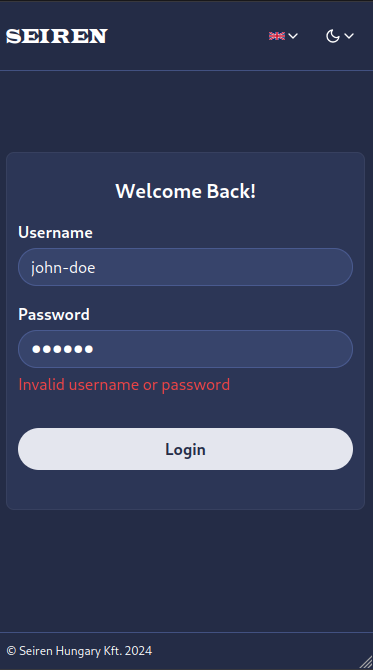
\includegraphics[clip, trim=0 30 0 0, height=0.4\textheight]{images/login_wrong_passwd.png}
        \caption{Hibás jelszó}
        \label{fig:login_wrong_passwd}
    \end{subfigure}
    \hfill
    \begin{subfigure}[b]{0.45\textwidth}
        \centering
        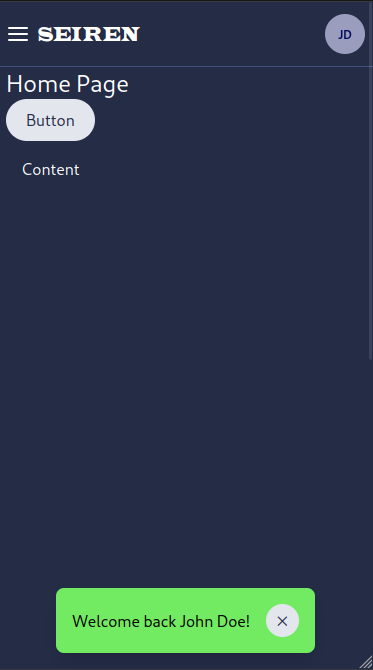
\includegraphics[height=0.4\textheight]{images/login_successful.png}
        \caption{Sikeres bejelentkezés}
        \label{fig:login_successful}
    \end{subfigure}
    \caption{Bejelentkezés}
    \label{fig:login}
\end{figure}

\subsection{Profil infó oldal, EntraPass adatok(09.15.)}

A mai napot a profil infó oldal (\ref{fig:profile_info}.~ábra) implementálásával kezdtem. Itt tekinthetik meg a
felhasználók az adataikat.

\begin{figure}[ht]
  \centering
  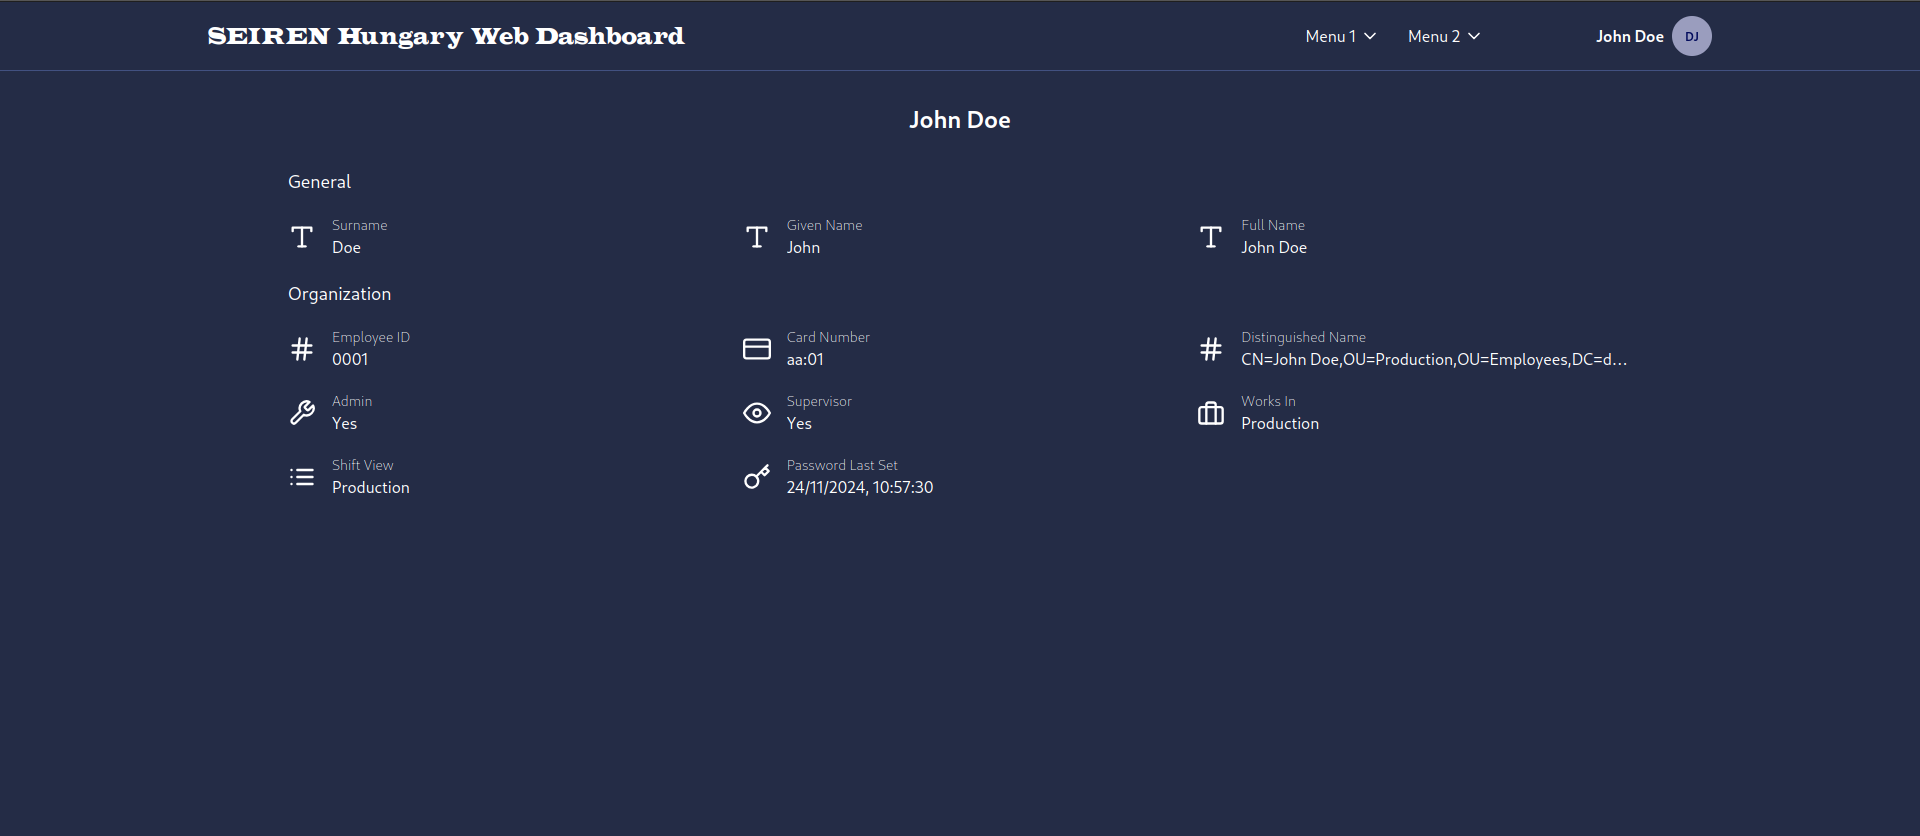
\includegraphics[width = 0.8\textwidth]{images/profile_info.png}
  \caption{/account/profile oldal}
  \label{fig:profile_info}
\end{figure}

\subsubsection*{EntraPass adatok}

Ezt követően az EntraPass Special Edition szoftverrel kezdtem el ismerkedni, amelyet a
cég a beléptetési adatok rögzítéséhez használ.
Mint kiderült, ez a szoftver (illetve ez a kiadás) egy beágyazott adatbázissal
dolgozik, melyet ”kívülről” nem lehet elérni. Ez azt jelenti, hogy az alkalmazás nem fog tudni kéréseket küldeni az
EntraPass szervernek. Az egyetlen mód adatok kinyerésére a szoftverből a riport generálás, mely egy adott időintervallumban
keletkezett beléptetési adatokat exportálja .csv formátumba. A riport generálást automatizálni lehet. Például be lehet
állítani, hogy a hét minden napján, 23:59-kor generáljon egy riportot az adott nap adataiból. \\

A megoldás tehát, az lesz, hogy az EntraPass szerver automatikusan generálja a riportokat, melyeket valamilyen fájlszinkronizációs
programmal eljuttat az alkalmazást futtató szerverre. Az alkalmazás figyelni fogja az adott könyvtárakat, majd
a hozzáadott .csv fájlokat feldolgozza és a saját adatbázisába menti. \\

\textit{CSV adatok, adatbázisba mentett adatok}

Az EntraPass által generált riportok formája \aref{fig:csv_format}.~ábrán látható.
Ebből a formátumból kell majd \aref{fig:card_usages_schema}.~ábrán megjelölt séma szerint menteni az adatokat az adatbázisba. Idő közben a követelmények bővültek
azzal, hogy egy esetleges vészhelyzet esetén az alkalmazással az éppen gyárban
tartózkodó személyeket is meg lehessen jeleníteni. Ehhez két további táblát is létre
kell majd hozzak. Megfigyelhető, hogy az \inltxt{emergency_card_usages} tábla nem tartalmaz HR
azonosítót, helyette csak a kártyaszámot. Ez több szempontból is indokolt. Egyrészt,
HR azonosítója csak a cég által alkalmazott személyeknek van, egy vészhelyzet esetén pedig minden személy helyzetét tudni kell.
Másrészt, az AD szerverrel való kommunikáció csak egy plusz hibaforrást jelentene, amely vészhelyzet esetén nem kívánatos.

\begin{figure}[ht]
  \centering
  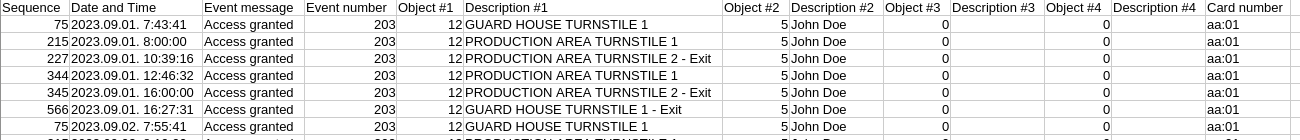
\includegraphics[width = 0.8\textwidth]{images/csv.png}
  \caption{Riport csv}
  \label{fig:csv_format}
\end{figure}

\begin{figure}[ht]
  \centering
  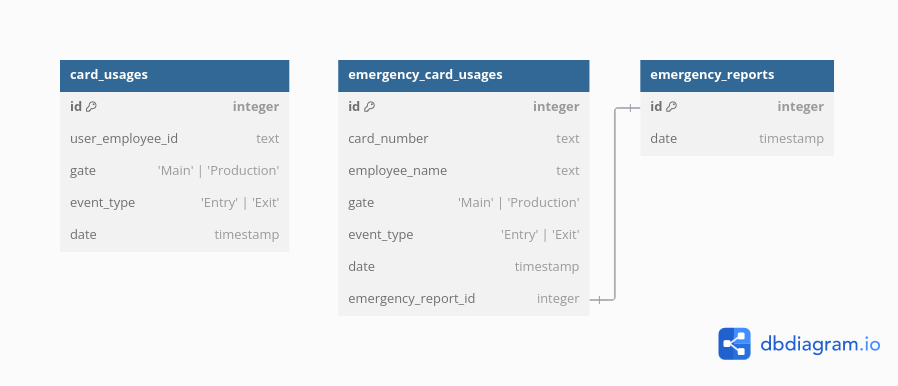
\includegraphics[clip, trim=0 50 0 0, width = 0.8\textwidth]{images/card_usages_schema.png}
  \caption{Kártyahasználati adatok, adatbázis séma}
  \label{fig:card_usages_schema}
\end{figure}


\section{Harmadik Hét}

\subsection{EntraPass adatok feldolgozása (09.18.)}

A tegnapi napon megtervezettek szerint, ma az EntraPass adatok alkalmazás oldali feldolgozását
implementáltam. Először megírtam a \inlts{reportFileParserService}-t, amely a chokidar könyvtárat
felhasználva figyeli a – környezeti változóként megadott – „daily reports” és „emergency reports”
mappákat. Amint egy új CSV fájl-t a mappák valamelyikébe másolunk, a service a csv-parser
könyvtár segítségével parseolja azt, majd az átalakított (\inlts{ParsedDailyReportRow}, illetve
\inlts{ParsedEmergencyReportRow} típusok) adatokkal meghívja a \inlts{cardUsageService}
\inlts{insertParsedDailyReportRows} vagy \inlts{insertParsedEmergencyReportRows} metódusát. Ezek
a metódusok szintén végeznek némi átalakítást az adatokon majd az adatbázis megfelelő tábláiba
tárolják azokat.

\subsection{Kártyahasználati adatok átalakítása a munkaidő kimutatás oldal\\ betöltésekor (1) (09.19.)}

Egyeztetések alapján, a munkaidő kimutatás (timesheet) oldalnak két nézete lehet az alapján, hogy az
alkalmazott milyen beosztásban dolgozik: termelési, illetve irodai nézet. A két nézethez különböző
adatokra van szükség. A timesheet oldal betöltésekor az alkalmazás két dátum közötti \inlts{cardUsage}
rekordokat lekérdezi, majd átalakítja az alábbi két típus valamelyikébe.

\FloatBarrier
\begin{minted}[bgcolor=codebg, breaklines, breakanywhere, fontsize=\small]{typescript}
// lib/types/shiftViewData.ts
export type ProductionShiftViewData = {
    shifts: {
        startDay: Date;
        endDay: Date;
        firstProductionEntry: Date;
        lastProductionExit: Date;
        totalWorkedTimeMs: number;
        totalInFactoryTimeMs: number;
        totalInProductionTimeMs: number;
        overtimeMs: number;
        inFactoryIntervals: {
            startDate: Date;
            endDate: Date;
            timeInFactoryMs: number;
            totalProductionTimeMs: number;
            inProductionIntervals: {
                startDate: Date;
                endDate: Date;
                timeInProductionMs: number;
            }[];
        }[];
    }[];
    numberOfShifts: number;
    totalTimeWorkedMs: number;
    averageTimeWorkedMs: number;
    totalTimeInFactoryMs: number;
    averageTimeInFactoryMs: number;
    totalTimeInProductionMs: number;
    averageTimeInProductionMs: number;
    totalOvertimeMs: number;
    cardUsageAnomalies: {
        cardUsageIndex: number;
        error: string;
    }[];
};

export type OfficeShiftViewData = {
    shifts: {
        day: Date;
        firstFactoryEntry: Date;
        lastFactoryExit: Date;
        timeWorkedMs: number;
        overtimeMs: number;
    }[];
    numberOfShifts: number;
    totalTimeWorkedMs: number;
    averageTimeWorkedMs: number;
    mostTimeWorkedMs: number;
    leastTimeWorkedMs: number;
    totalOvertimeMs: number;
};
\end{minted}

A tervezés után el is elkezdtem implementálni ezt a működést. Az átalakítást két részre bontva, a
rekordokat először \inlts{Production/OfficeShiftVewDataIntervalDates} típusba alakítom.
Ezekben a típusokban csak a kezdő és záró dátumok találhatók. A későbbi, számított attribútumokat
két másik függvényben számolom ki.

\FloatBarrier
\begin{minted}[bgcolor=codebg, breaklines, breakanywhere, fontsize=\small]{typescript}
// lib/types/shiftViewData.ts
export type ProductionShiftViewDataIntervalDates = {
    shifts: {
        startDay: Date;
        endDay: Date;
        inFactoryIntervals: {
            startDate: Date;
            endDate: Date;
            inProductionIntervals: {
                startDate: Date;
                endDate: Date;
            }[];
        }[];
    }[];
    cardUsageAnomalies: {
        cardUsageIndex: number;
        error: string;
    }[];
};

export type OfficeShiftViewDataIntervalDates = {
    shifts: {
        day: Date;
        firstFactoryEntry: Date;
        lastFactoryExit: Date;
    }[];
};
\end{minted}

\subsection{Kártyahasználati adatok átalakítása a munkaidő kimutatás oldal\\ betöltésekor (2) (09.20.)}

Először befejeztem a rekordok \inlts{Production/OfficeShiftVewDataIntervalDates}
típusba alakítását. Ezt követően a \inlts{getProductionShiftViewData}, illetve a
\inlts{getOfficeShiftViewData} függvényeket írtam meg, melyek a számított adatokkal egészítik ki a
\inlts{Production/OfficeShiftVewDataIntervalDates} típusú objektumokat
\inlts{Production/OfficeShiftVewData} típusú objektumokká.

\subsection{Timesheet oldal - dátum intervallum beviteli mező, adatok kérése (09.21.)}

A timesheet oldallal kezdtem el foglalkozni. Első körben egy dátum intervallum beviteli mezőt
szerettem volna implementálni, hogy a munkaidő adatokat a felhasználók dátum szerint tudják szűrni.
Mivel, a Skeleton UI Toolkit nem tartalmaz ilyen komponenst, igy a \href{https://vanilla-calendar.pro/}{vanilla-calendar-pro} könyvtárra
esett a választásom. Egyetlen hátulütője az volt, hogy a naptár színeit csak úgy tudtam testreszabni,
hogy a könyvtárhoz tartozó CSS fájlokat felülírtam a saját CSS fájljaimmal. A végeredmény \aref{fig:calendars}.~ábrán
látható.\\

\begin{figure}[ht]
    \centering
    \begin{subfigure}[b]{0.45\textwidth}
        \centering
        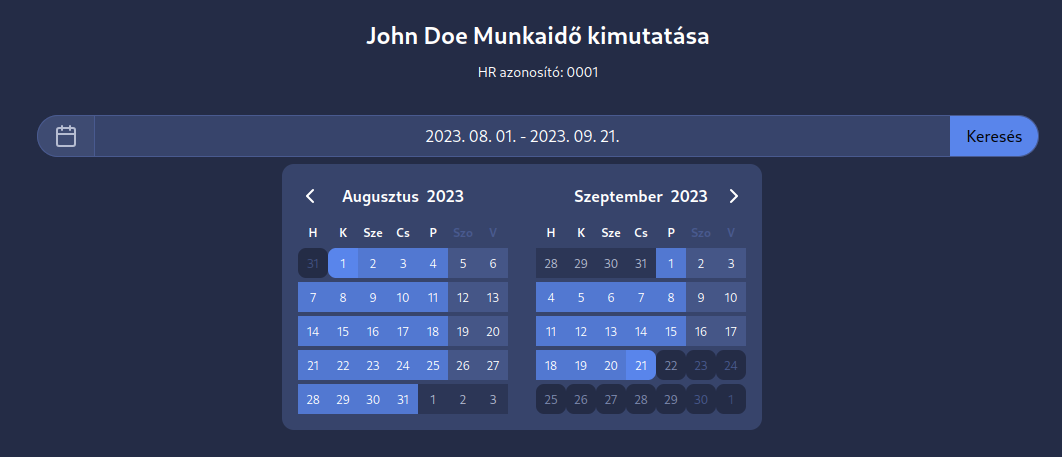
\includegraphics[clip, trim=25 0 25 0, width=1\textwidth]{images/calendar-dark.png}
        \caption{Sötét mód}
        \label{fig:calendar_dark}
    \end{subfigure}
    \hfill
    \begin{subfigure}[b]{0.45\textwidth}
        \centering
        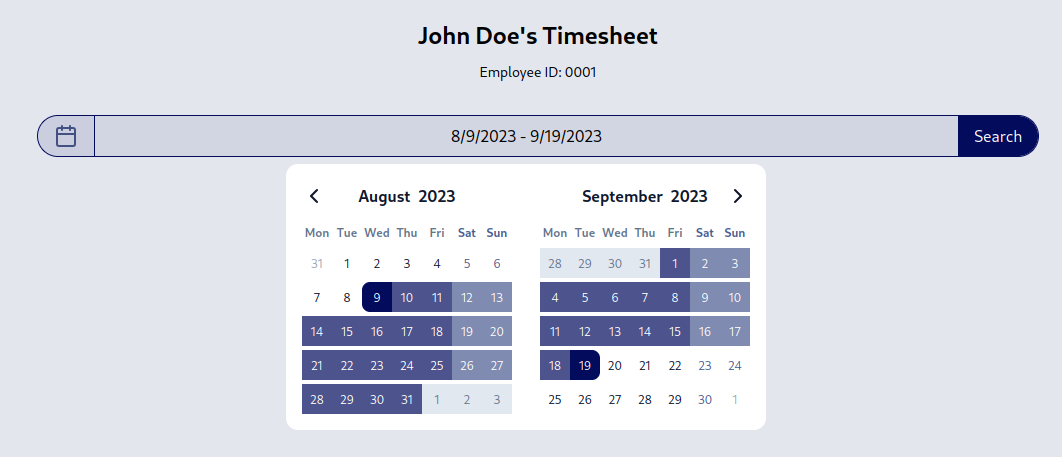
\includegraphics[clip, trim=25 0 25 0, width=1\textwidth]{images/calendar-light.png}
        \caption{Világos mód}
        \label{fig:calendar_light}
    \end{subfigure}
    \caption{Dátum intervallum beviteli mező}
    \label{fig:calendars}
\end{figure}

Ezt követően létrehoztam egy \inltxt{/api/shift-view-data/search} API útvonalat, valamint az ennek
megfelelő \inltxt{apiClient.fetchShiftViewData()} függvényt, mely utóbbit a böngésző a „keresés”
gombra kattintva meghív (\ref{fig:timesheet_search}.~ábra). E mellett az oldal PageLoad függvényét is megírtam, hogy az első
betöltéskor – SSR-et alkalmazva – az oldal már tartalmazza az aktuális havi adatokat.

\begin{figure}[ht]
  \centering
  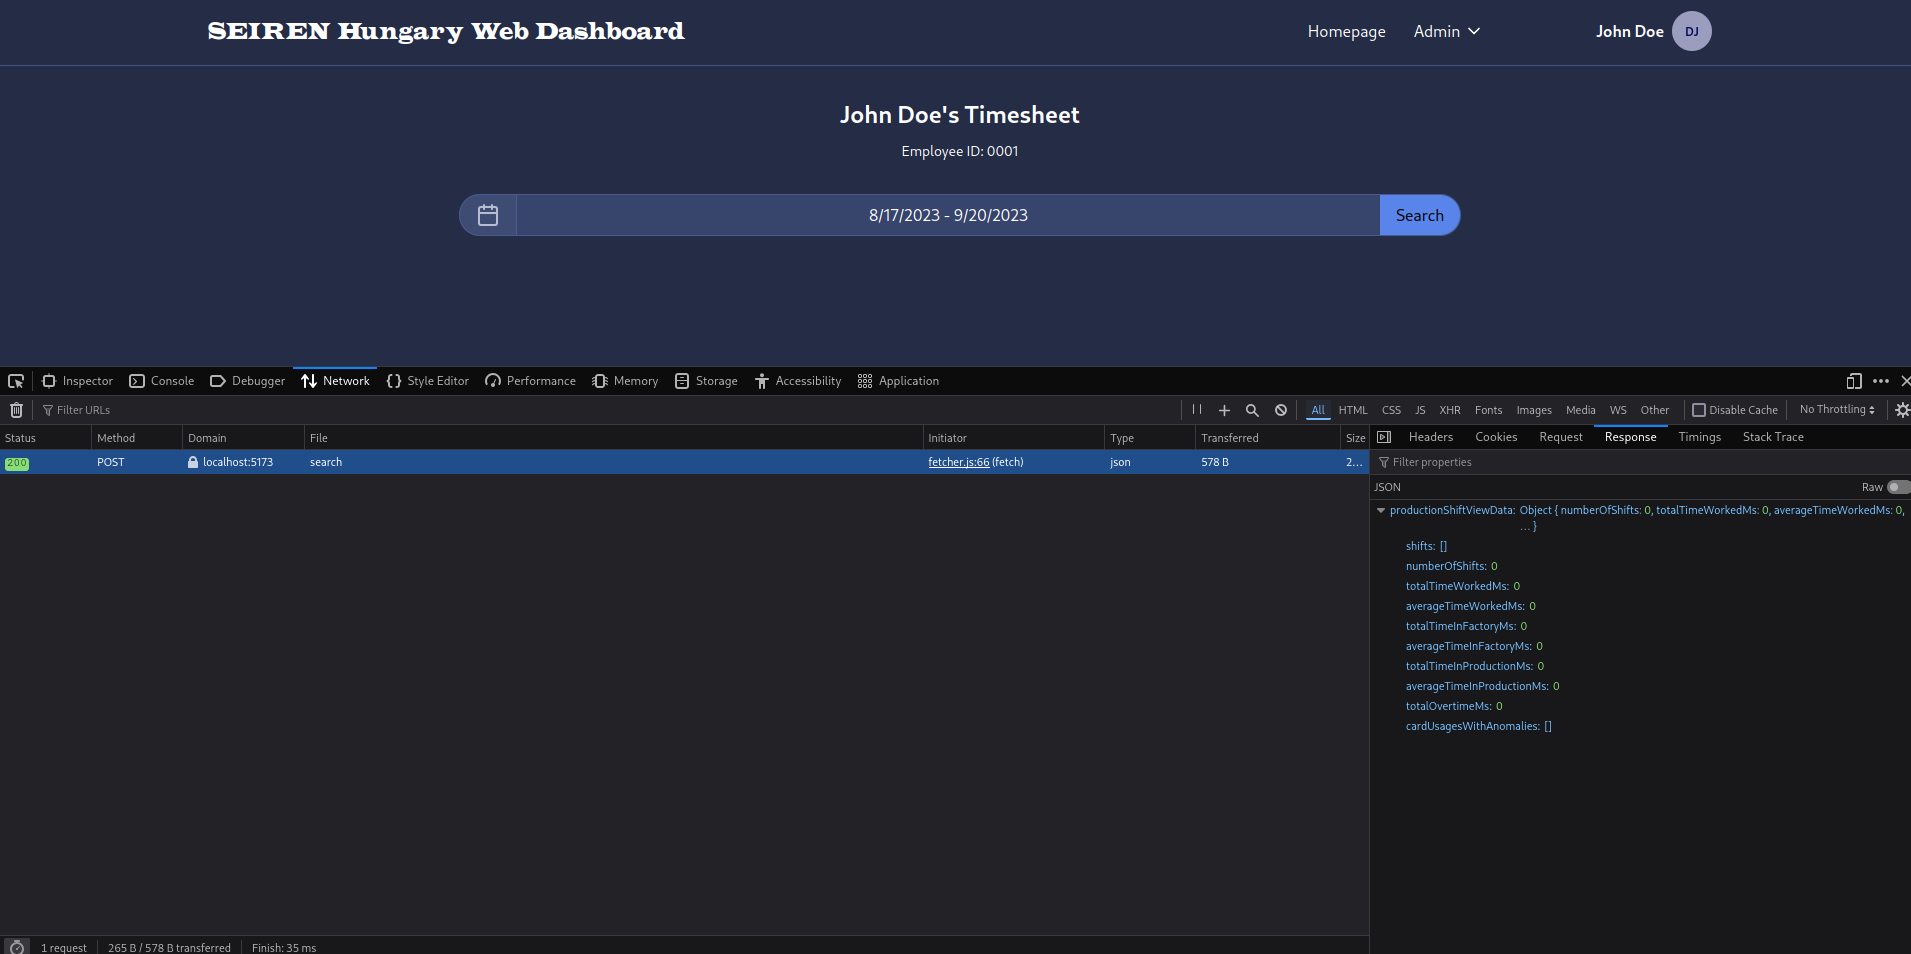
\includegraphics[width = 0.8\textwidth]{images/timesheet_search.png}
  \caption{/api/shift-view-data/search API útvonal}
  \label{fig:timesheet_search}
\end{figure}

\subsection{PaginatedShiftTreeView komponens (09.22.)}

A timesheet oldalra egy olyan "lapozható" komponenst implementáltam, amellyel a
felhasználó a keresett intervallumban szereplő munkaidő adatokat
(\inltxt{Office|ProductionShiftViewData.shifts}) tudja megtekinteni napokra bontva. Termelés
nézetben (\ref{fig:production_view}.~ábra) a komponens lenyitható füleket tartalmaz, míg irodai nézet esetében (\ref{fig:office_view}.~ábra) a komponens csak
egyszintes.

\begin{figure}[ht]
    \centering
    \begin{subfigure}[b]{0.8\textwidth}
        \centering
        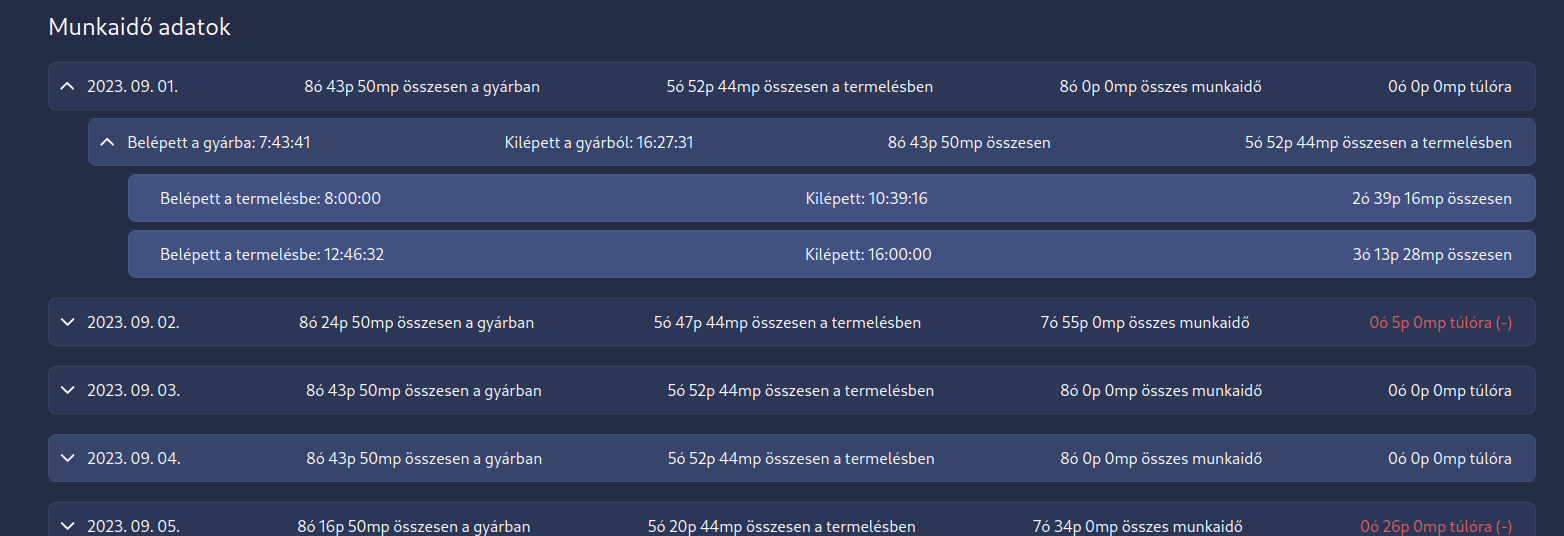
\includegraphics[width=\textwidth]{images/production_view.png}
        \caption{Termelés nézet}
        \label{fig:production_view}
    \end{subfigure}

    \vspace{1em} % Adjust vertical space between images

    \begin{subfigure}[b]{0.8\textwidth}
        \centering
        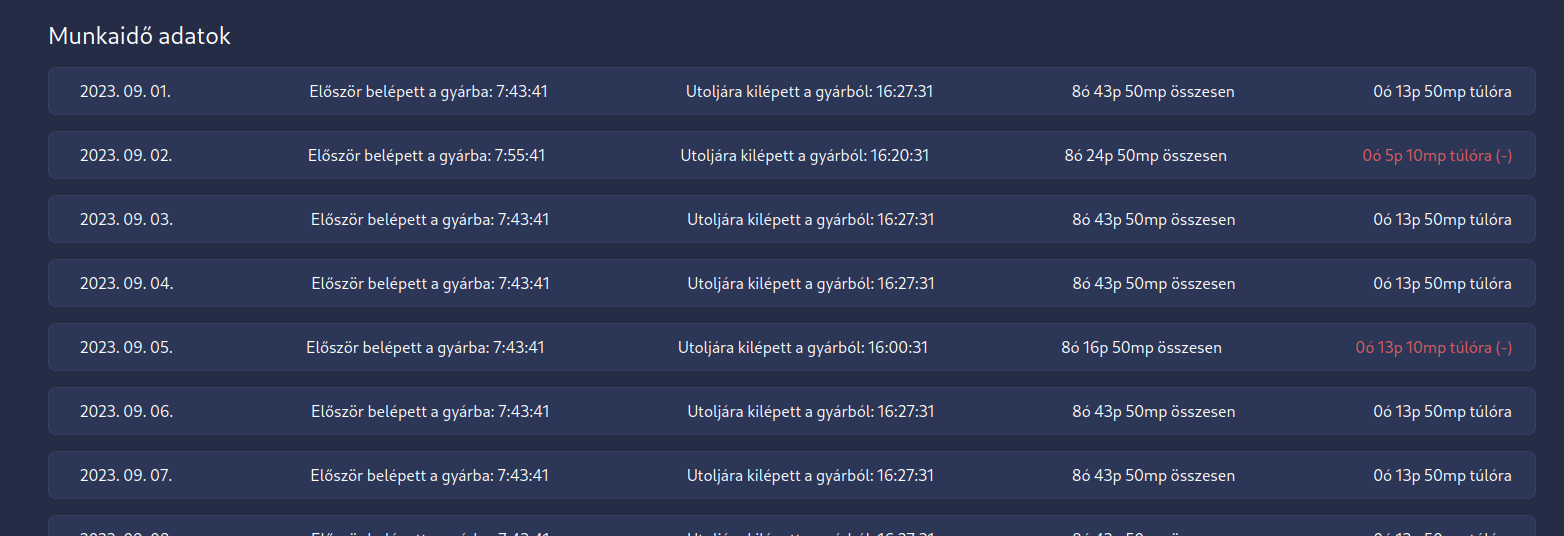
\includegraphics[width=\textwidth]{images/office_view.png}
        \caption{Irodai nézet}
        \label{fig:office_view}
    \end{subfigure}

    \caption{PaginatedShiftTreeView komponens}
    \label{fig:paginated_shift_tree_view}
\end{figure}

\section{Negyedik Hét}

\subsection{Kártyahasználati adatok táblázat (09.25.)}

Egy DataNotFound komponens implementálásával kezdtem, amely akkor jelenik meg a timesheet
oldalon, ha az adott intervallumban nem található adat.\\

Ez után, egy olyan lapozható táblázatot adtam hozzá az oldalhoz, melyben a kártyahasználati adatokat
lehet megtekinteni (\ref{fig:card_usages_table}.~ábra).

\begin{figure}[ht]
  \centering
  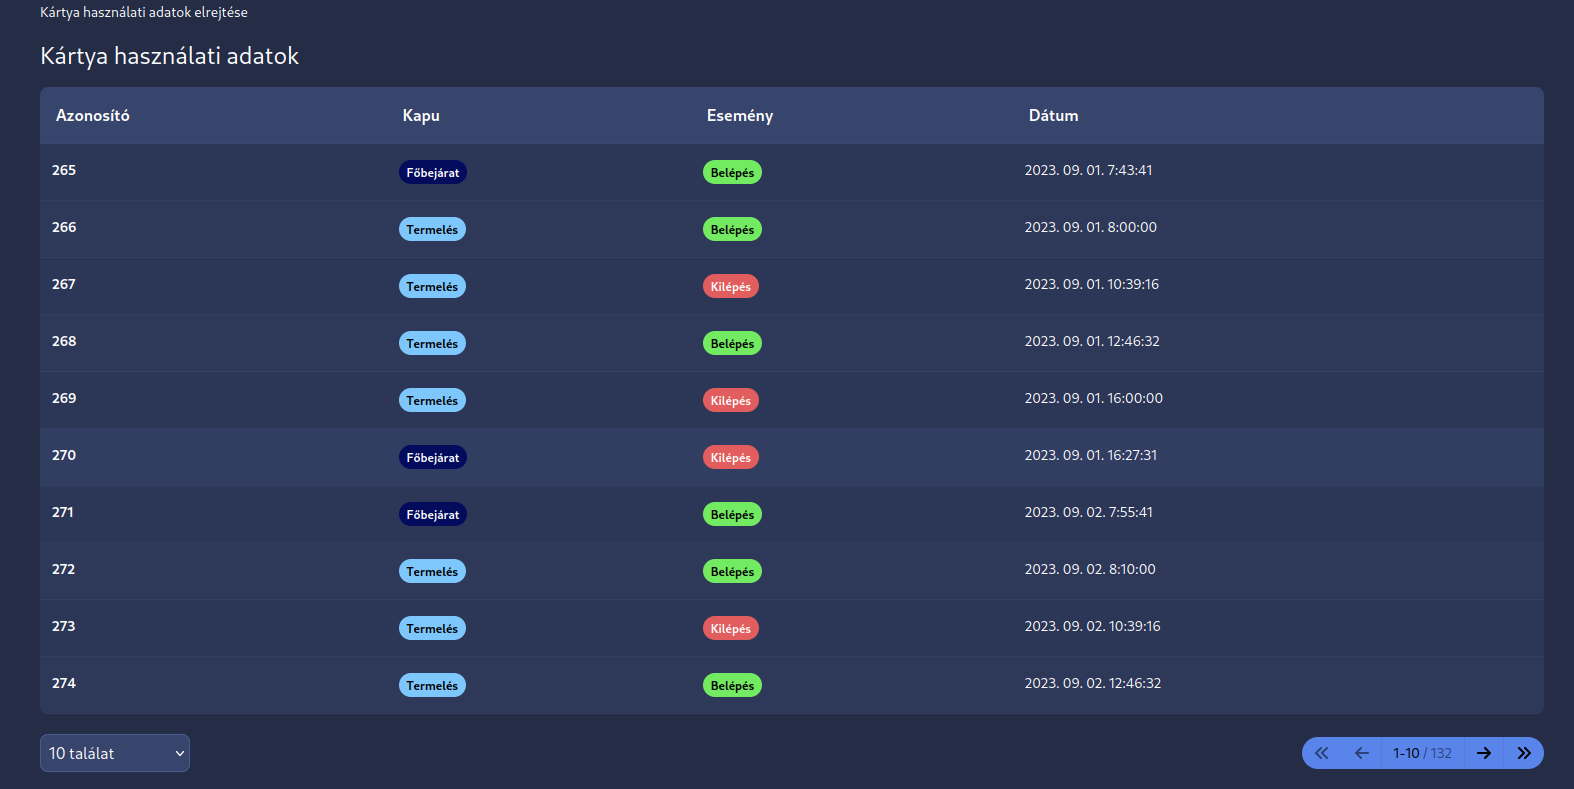
\includegraphics[width = 0.8\textwidth]{images/card_usages_table.png}
  \caption{Kártyahasználati adatok táblázat}
  \label{fig:card_usages_table}
\end{figure}

\subsection{StatCards komponens, hiba javítása (09.26.)}

A timesheet oldalra írtam egy olyan komponenst, amelyben "kártyákban" szerepelnek a lekért
munkaidő adatokhoz (\inltxt{Office|ProductionShiftViewData}) tartozó statisztikák (\ref{fig:stat_cards}.~ábra). Például:
dolgozott napok száma, összes túlóra, összes dolgozott idő, stb.\\

\begin{figure}[ht]
  \centering
  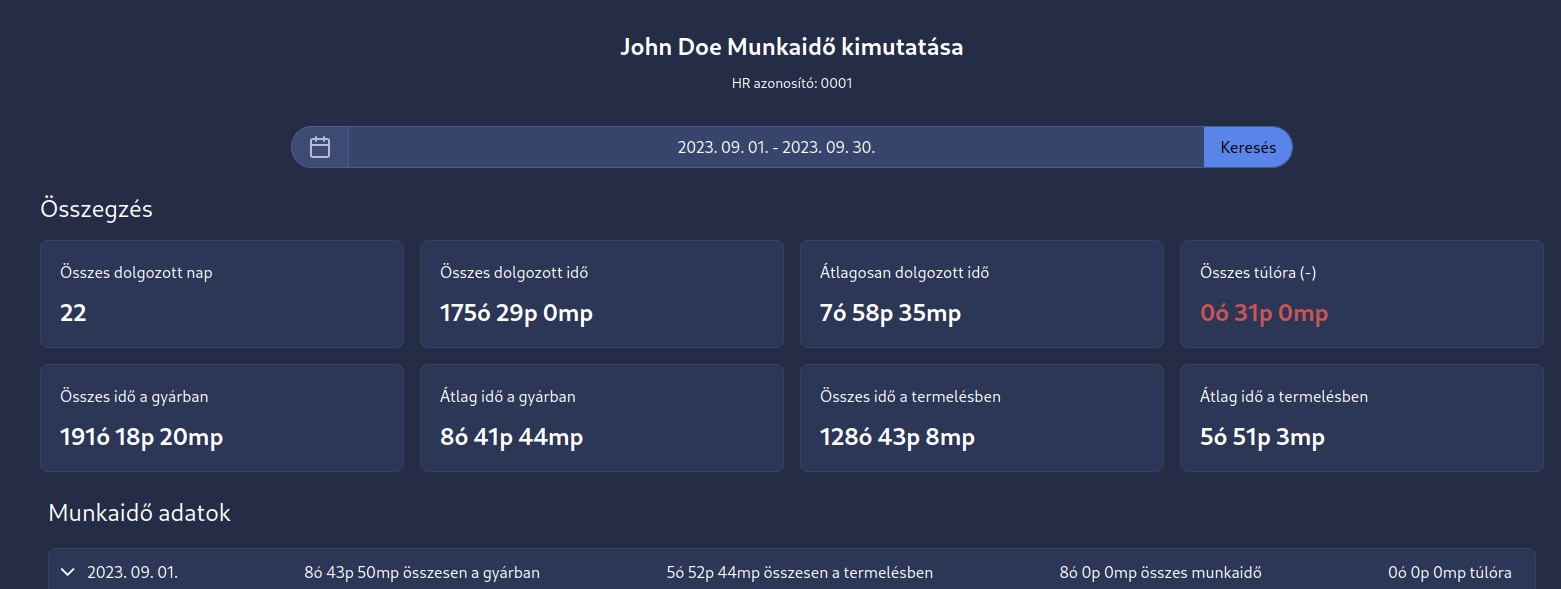
\includegraphics[width = 0.8\textwidth]{images/stat_cards.png}
  \caption{StatCards komponens}
  \label{fig:stat_cards}
\end{figure}

Ezt követően egy hibát javítottam ki, mely a
\inlts{cardUsageUtils.getOffice|ProductionShiftViewData} függvényekben lépett/léptek fel,
valamint írtam néhány tesztet is hozzájuk.

\subsection{MultilineChart komponens (09.27.)}

A timesheet oldalra implementáltam a \href{https://layercake.graphics/}{layercake} library segítségével egy több vonalt tartalmazó
diagramot. Ezen a diagramon (\ref{fig:chart}.~ábra) napokra bontva szerepel az összes dolgozott idő, a túlóra, valamint -
termelési nézet esetén - az összes gyárban, és termelésben töltött idő.

\begin{figure}[ht]
  \centering
  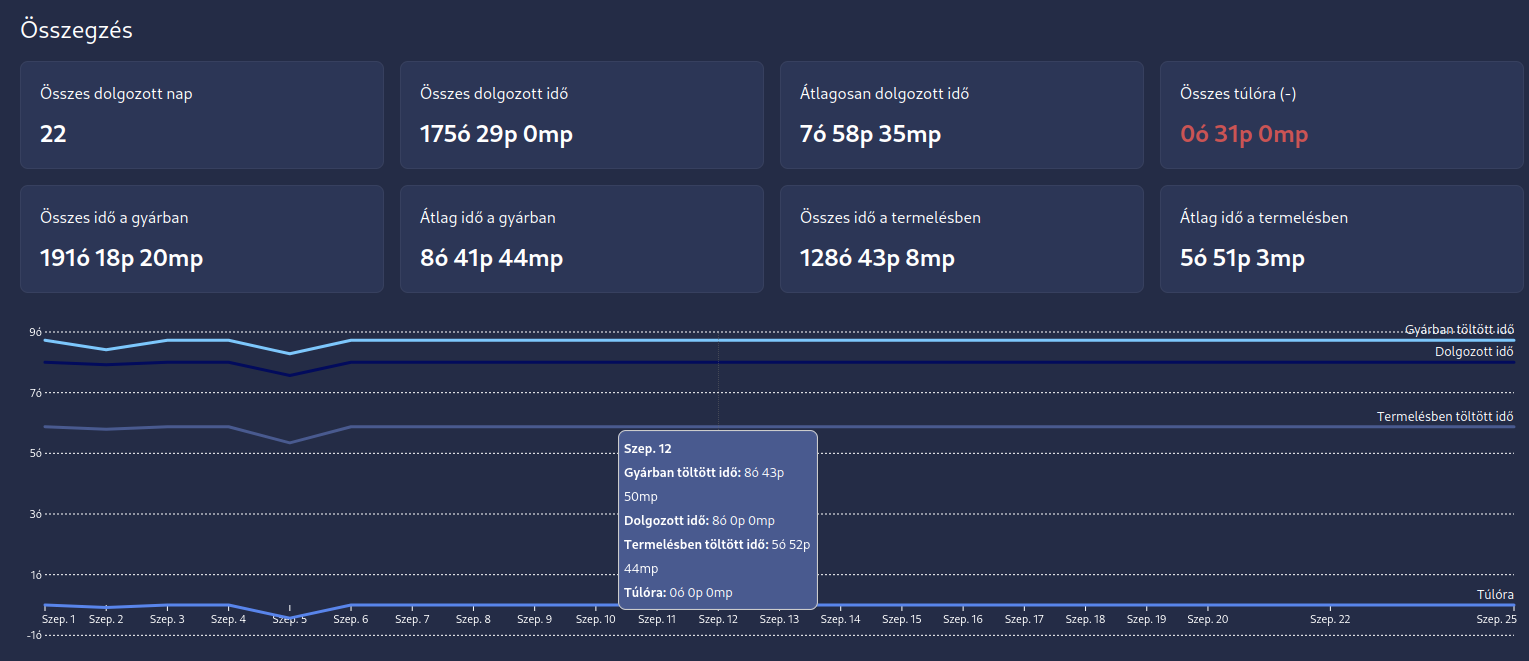
\includegraphics[width = 0.8\textwidth]{images/chart.png}
  \caption{MultiLineChart komponens}
  \label{fig:chart}
\end{figure}

\subsection{PDF-be exportálás (09.28.)}

A munkaidő adatok PDF-ként való exportálását
oldottam meg a \href{https://www.npmjs.com/package/jspdf}{jspdf} könyvtár segítségével. A
felhasználó kiválaszthatja egy checkbox
segítségével (\ref{fig:export_component}.~ábra), hogy az exportált pdf (\ref{fig:report_pdf}.~ábra) tartalmazza e a
kártyahasználati adatokat, valamint termelési
nézetben a lenyíló fülek tartalmát.

\begin{figure}[ht]
  \centering
  
\includegraphics[width=0.4\textwidth]{images/export.png}
  \caption{Export komponens}
  \label{fig:export_component}
\end{figure}

\begin{figure}[ht]
  \centering
  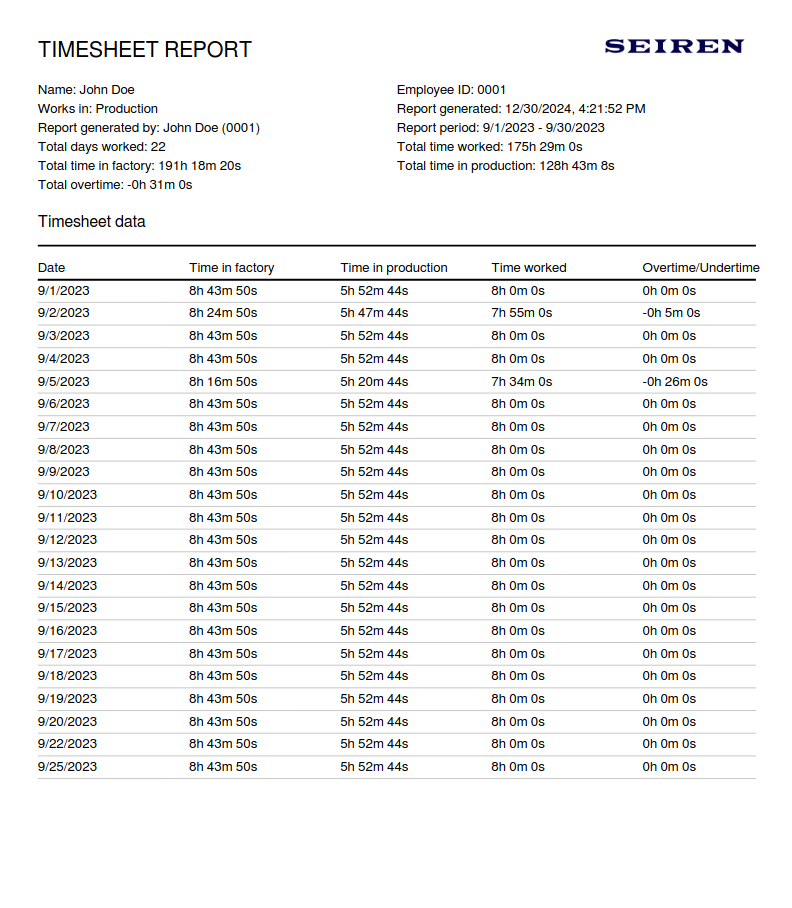
\includegraphics[width = 0.6\textwidth]{images/report_pdf.png}
  \caption{Exportált PDF}
  \label{fig:report_pdf}
\end{figure}

\subsection{XLSX-be exportálás (09.29.)}

A tegnapi nap mintájára, ma a munkaidő adatok XLSX-ként való exportálását implementáltam az
\href{https://www.npmjs.com/package/exceljs}{exceljs} könyvtár segítségével (\ref{fig:report_xlsx}.~ábra).

\begin{figure}[ht]
  \centering
  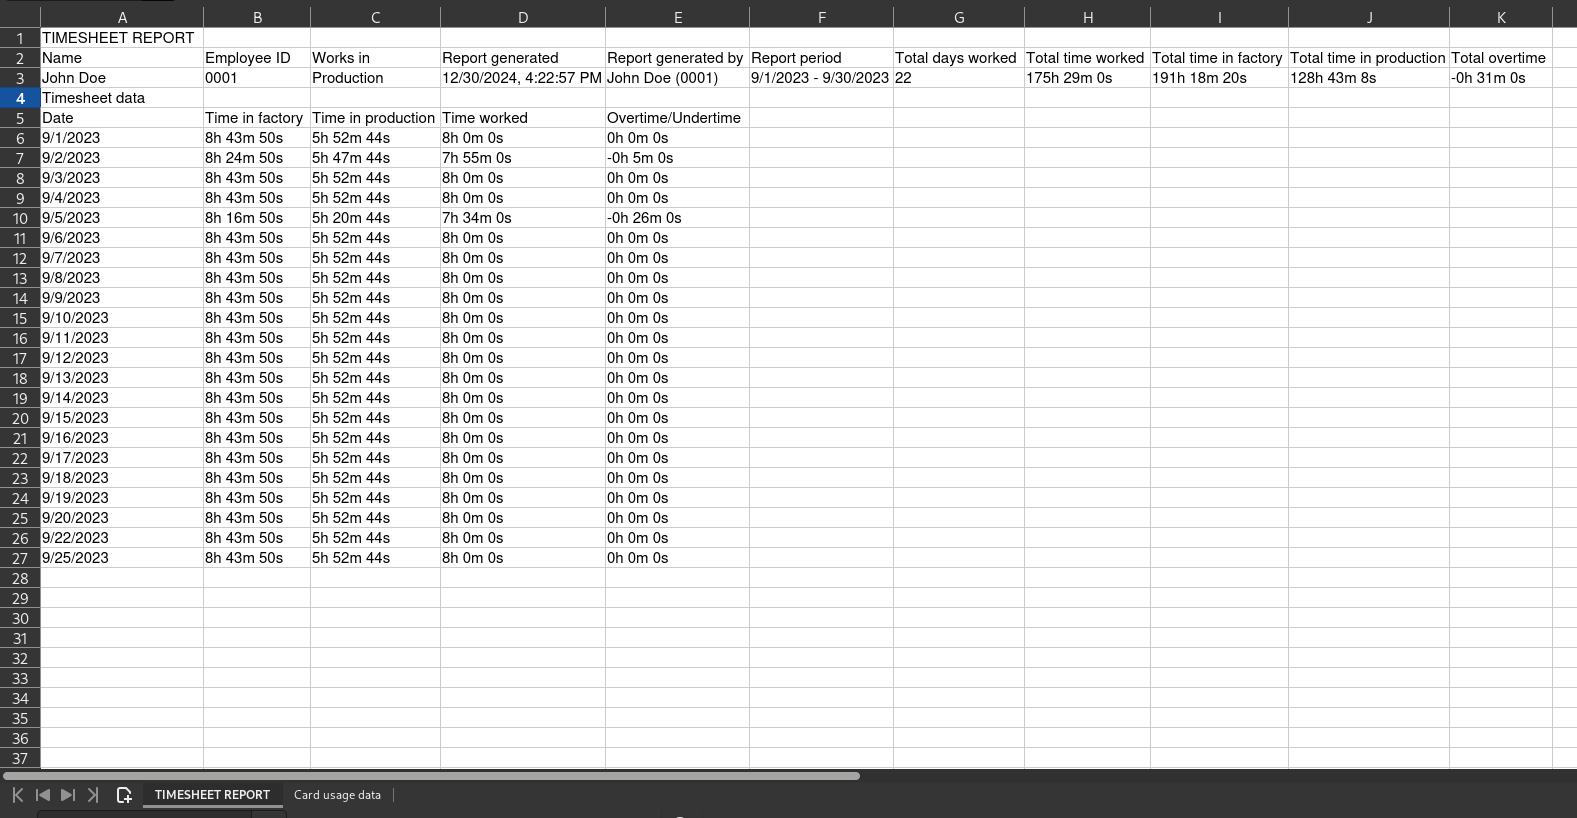
\includegraphics[width = 0.8\textwidth]{images/report_xlsx.png}
  \caption{Exportált XLSX}
  \label{fig:report_xlsx}
\end{figure}

\section{Ötödik Hét}

\subsection{/admin/employees oldal (backend) (10.16.)}

Az adminisztrátorok számára elérhető funkciók implementálását kezdtem meg. Az első funkció a
dolgozók keresése és a találatok táblázatos megjelenítése. Elkészítettem a \inltxt{searchUsers()}
függvényt az Active Directory service-hez, amely név, felhasználónév (\inltxt{sAMAccountName}), HR ID és
kártyaszám alapján teszi lehetővé a keresést az Active Directory rekordjai között. Mivel az Active
Directory nem támogatja a lapozást (pagination), ezt a kliensoldalon fogom megvalósítani.\\

Ezt követően létrehoztam a \inltxt{/api/users/search} végpontot, valamint implementáltam az ehhez
tartozó \inltxt{apiClient.searchUsers()} függvényt.


\subsection{/admin/employees oldal (10.17.)}

Elkészítettem a dolgozók táblázatát (\ref{fig:employees}.~ábra) tartalmazó \inltxt{/admin/employees} oldalt. A táblázat fejlécében a
felhasználó módosíthatja a rendezési beállításokat, és az adott mezőhöz tartozó szűrőt is. Az utolsó
oszlopban három gomb található: a bal oldali a dolgozó munkaidő-adatait megjelenítő oldalra, a
középső a dolgozó profiloldalára navigál, míg a jobb szélső gomb a dolgozó adatainak törlésére (\ref{fig:delete_employee}.~ábra) szolgál.
Ez a törlés nem érinti az Active Directory-ban tárolt felhasználói adatokat, csak a dashboard alkalmazás
adatbázisából távolítja el a kapcsolódó adatokat.

\begin{figure}[ht]
  \centering
  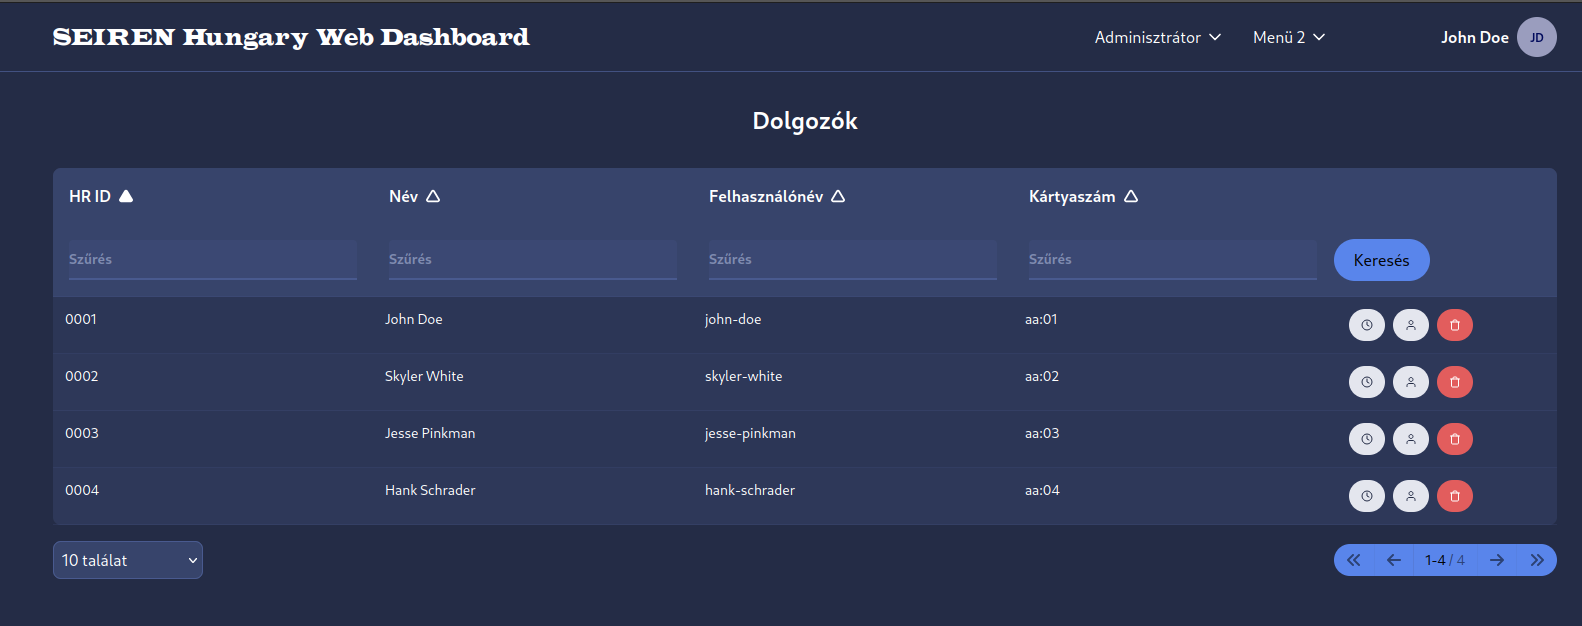
\includegraphics[width = 0.8\textwidth]{images/employees.png}
  \caption{/admin/employees táblázat}
  \label{fig:employees}
\end{figure}

\begin{figure}[ht]
  \centering
  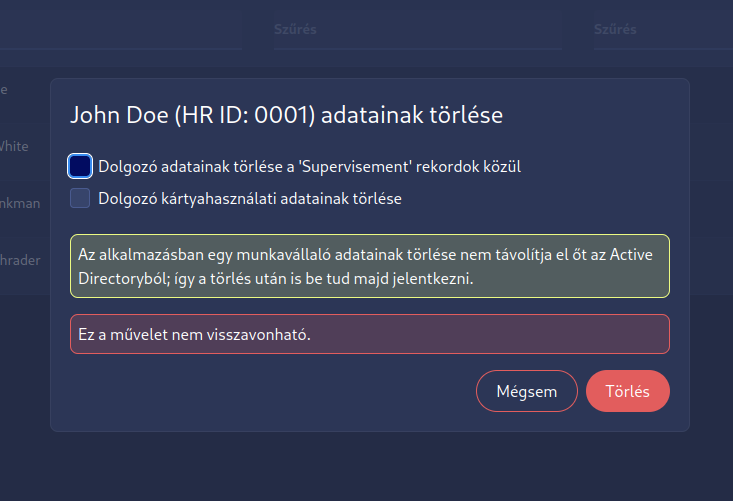
\includegraphics[width = 0.6\textwidth]{images/delete_employee.png}
  \caption{Dolgozó adatainak törlése}
  \label{fig:delete_employee}
\end{figure}

\subsection{Kártyahasználati adatok keresése (backend) (10.18.)}

A következő adminisztrátori funkció, a kártyahasználati adatok menedzselése került sorra. Első
lépésként implementáltam a cardUsage service \inltxt{getPaginatedCardUsages()} függvényét, a
következő paraméterekkel:

\FloatBarrier
\begin{minted}[bgcolor=codebg, breaklines, breakanywhere, fontsize=\small]{typescript}
export type CardUsageSearchParams = {
    pageNumber: number;
    pageSize: number;
    orderBy?: "id" | "userEmployeeId" | "gate" | "eventType" | "date";
    order?: "asc" | "desc";
    id?: string;
    userEmployeeId?: string;
    gate?: "Main" | "Production";
    eventType?: "Entry" | "Exit";
    startDate?: Date;
    endDate?: Date;
};
\end{minted}

Ezt követően elkészítettem a \inltxt{/api/admin/card-usages/search} végpontot és a hozzá tartozó
\inltxt{apiClient.searchPaginatedCardUsages} függvényt.

\subsection{/admin/card-usages oldal (10.19.)}

Elkezdtem dolgozni a kártyahasználati adatokat megjelenítő \inltxt{/admin/card-usages} oldalon.
Létrehoztam a kártyahasználati adatokat tartalmazó táblázatot (\ref{fig:admin_card_usages}.~ábra), amely hasonló a dolgozók
táblázatához, de az adatok itt szerveroldali pagination-el érhetők el, mivel az alklalmazás az adatokat
a saját adatbázisából kéri le. A táblázatban a felhasználó egyesével törölhet, módosíthat, új rekordokat
hozhat létre, illetve egyszerre több kijelölt rekordot is törölhet.

\begin{figure}[ht]
  \centering
  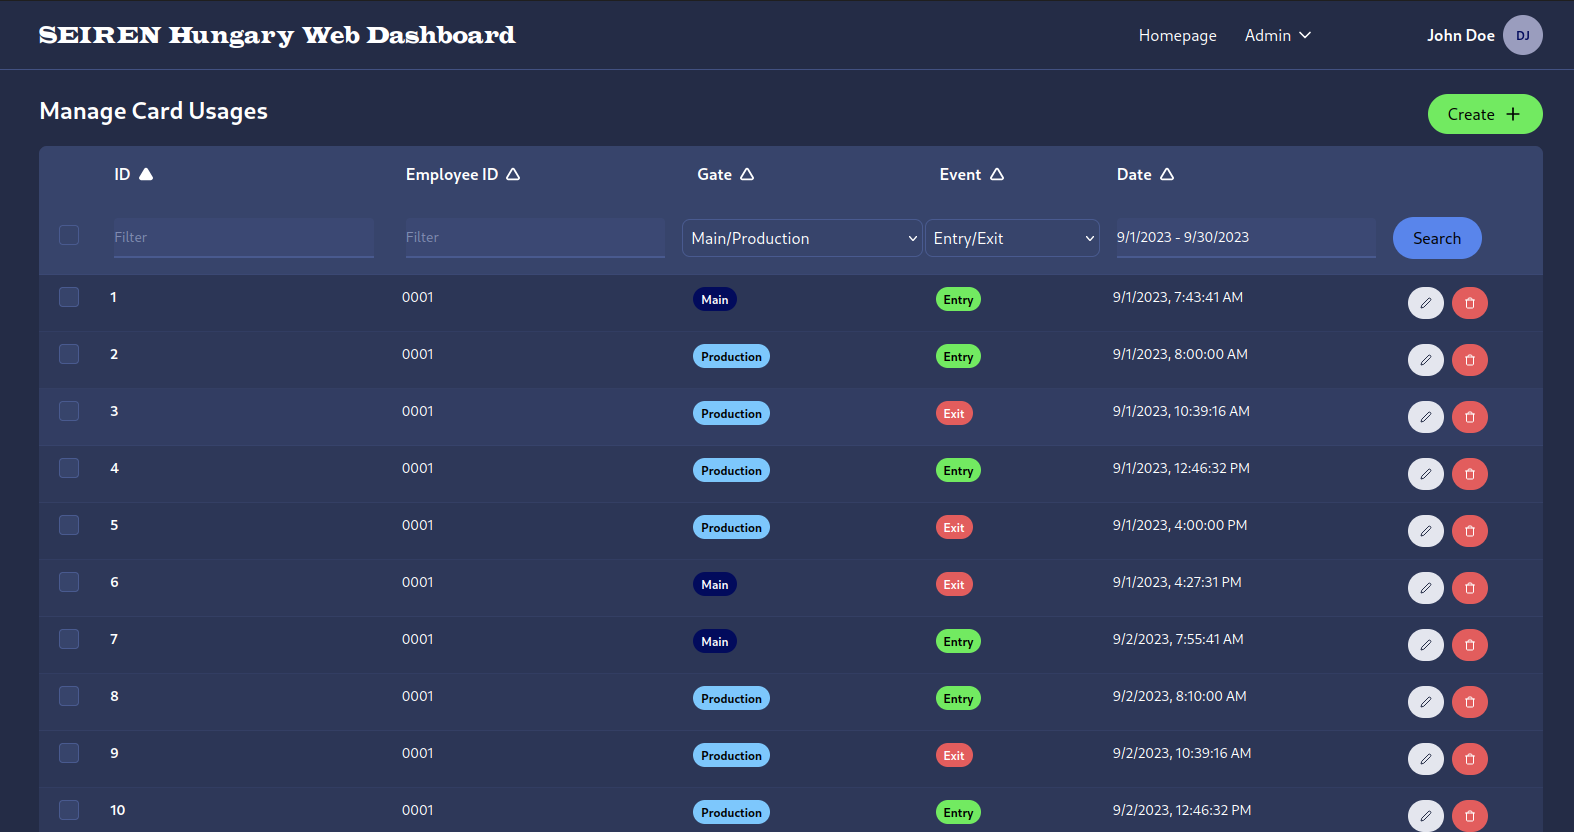
\includegraphics[width = 0.8\textwidth]{images/manage_card_usages.png}
  \caption{/admin/card-usages oldal}
  \label{fig:admin_card_usages}
\end{figure}

A nap végére sikerült befejezni a törlés funkciót (\ref{fig:delete_card_usage}.~ábra). \\


\begin{figure}[ht]
  \centering
  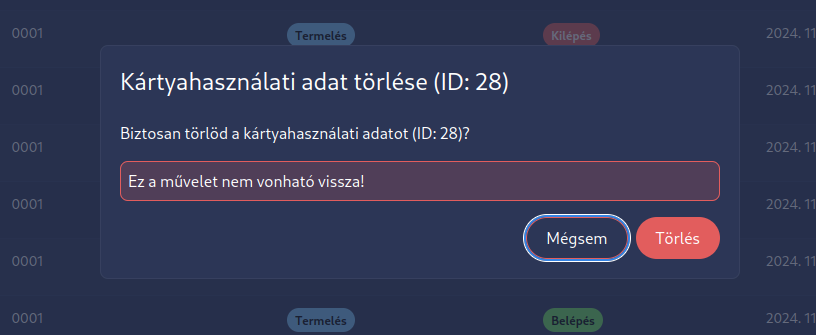
\includegraphics[clip, trim=40 0 40 0, width=0.5\textwidth]{images/delete_card_usage.png}
  \caption{Kártyahasználati adat törlése}
  \label{fig:delete_card_usage}
\end{figure}


A szerkesztési funkcióhoz tartozó modal
(modális ablak) implementálása során
problémába ütköztem: az általam
használt Vanilla Calendar Pro könyvtár időbeviteli mezője csak órák és percek megadását támogatja.
Ezért létrehoztam egy saját \inltxt{TimeInput} komponenst (\ref{fig:time_input}.~ábra), amely lehetővé teszi a másodperc értékének
megadását is.

\begin{figure}[ht]
  \centering
  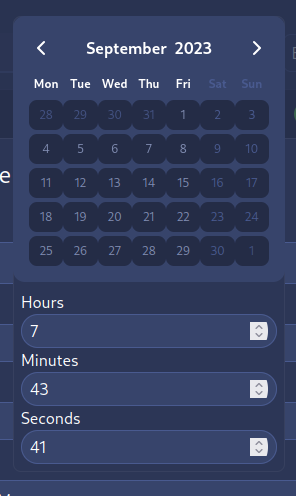
\includegraphics[width = 0.3\textwidth]{images/time_input.png}
  \caption{Dátum beviteli mező (TimeInput komponenssel)}
  \label{fig:time_input}
\end{figure}

\subsection{/admin/card-usages oldal befejezése (10.20.)}

A hátralévő funkciókat, vagyis a kártyahasználati adatok
szerkesztését, új rekordok létrehozását, valamint a kijelölt rekordok
törlését implementáltam frontend-, és backendoldalon. (\ref{fig:manage_card_usages}.~ábra)

\begin{figure}[ht]
    \centering
    \begin{subfigure}[b]{0.8\textwidth}
        \centering
        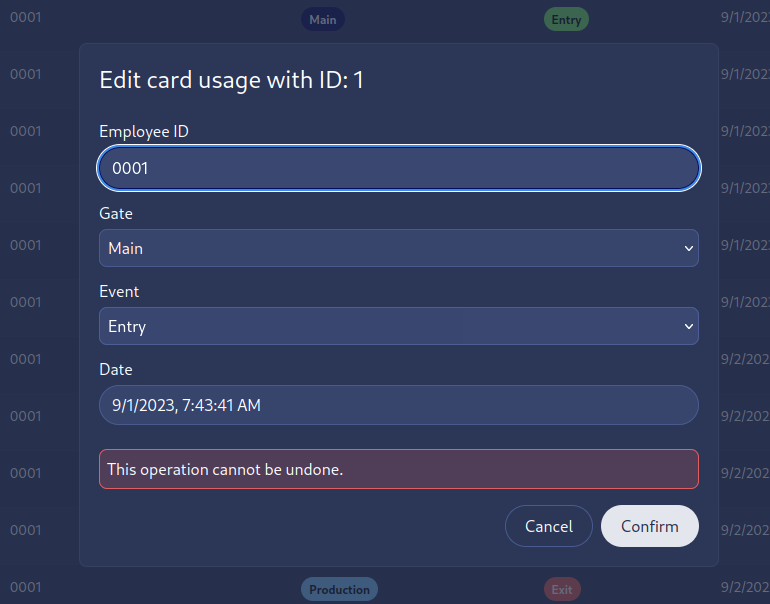
\includegraphics[width=0.8\textwidth]{images/card_usage_modify.png}
        \caption{Kártyahasználati adat módosítása modal}
        \label{fig:card_usage_modify}
    \end{subfigure}

    \vspace{1em} % Adjust vertical space between images

    \begin{subfigure}[b]{0.8\textwidth}
        \centering
        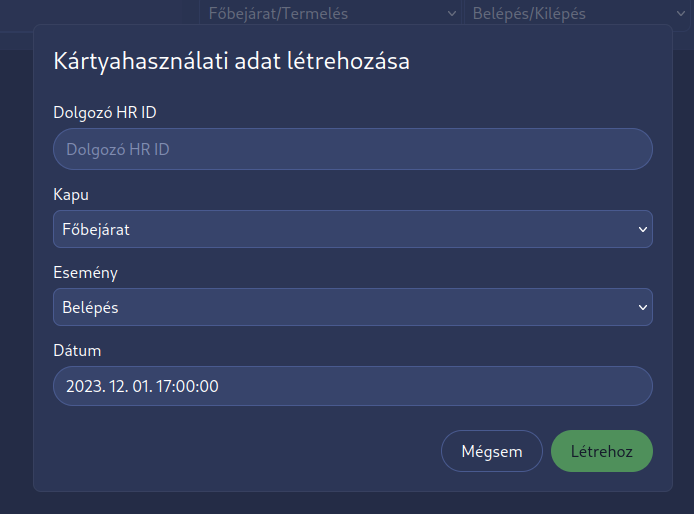
\includegraphics[width=0.8\textwidth]{images/create_card_usage.png}
        \caption{Kártyahasználati adat létrehozása modal}
        \label{fig:card_usage_create}
    \end{subfigure}

    \vspace{1em} % Adjust vertical space between images

    \begin{subfigure}[c]{0.8\textwidth}
        \centering
        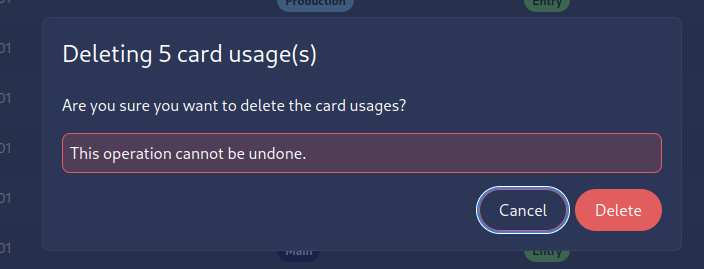
\includegraphics[width=0.6\textwidth]{images/card_usages_delete.png}
        \caption{Kiválasztott rekordok törlése modal}
        \label{fig:card_usages_delete}
    \end{subfigure}

    \caption{/admin/card-usages oldal funkciói}
    \label{fig:manage_card_usages}
\end{figure}

\section{Hatodik Hét}

\subsection{/admin/supervisement-groups oldal (BE) (10.23.)}

A következő adminisztrátorok számára elérhető funkción kezdtem el dolgozni, amely lehetővé teszi a
Supervisement (Felettesi) csoportok létrehozását és módosítását. Az adminisztrátor képes lesz
csoportokat létrehozni, például HR, IT, stb. részlegek számára, majd dolgozókat rendelhet hozzájuk
beosztottként vagy felettesként. A csoportokhoz rendelt dolgozók eltávolíthatók, a csoportok
átnevezhetők, illetve törölhetők lesznek.\\

Először létrehoztam a \inltxt{SupervisementGroups} adatbázis sémát (\ref{fig:sup_groups_schema}.~ábra), majd megírtam a supervisement
service következő függvényeit: \inltxt{createGroup}, \inltxt{getSupervisementGroupById}, \inltxt{deleteGroup},
\inltxt{renameGroup}, \inltxt{getPaginatedSupervisementGroups}. Ezt követően az ezekhez a
függvényekhez tartozó \inltxt{/api} végpontokat kezdtem el írni.

\begin{figure}[ht]
  \centering
  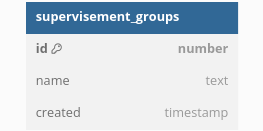
\includegraphics[width = 0.3\textwidth]{images/sup_groups_schema.png}
  \caption{supervisement\_groups adatbázis séma}
  \label{fig:sup_groups_schema}
\end{figure}

\subsection{/admin/supervisement-groups oldal (10.24.)}

Befejeztem a tegnap megkezdett \inltxt{/api} végpontok megírását, majd az azoknak megfelelő \inltxt{apiClient}
függvényeket írtam meg. Végül az \inltxt{/admin/supervisement-groups} oldalt kezdtem el
implementálni (\ref{fig:sup_groups}.~ábra), amely egy táblázatot tartalmaz a létrehozott supervisement csoportokról.

\begin{figure}[ht]
  \centering
  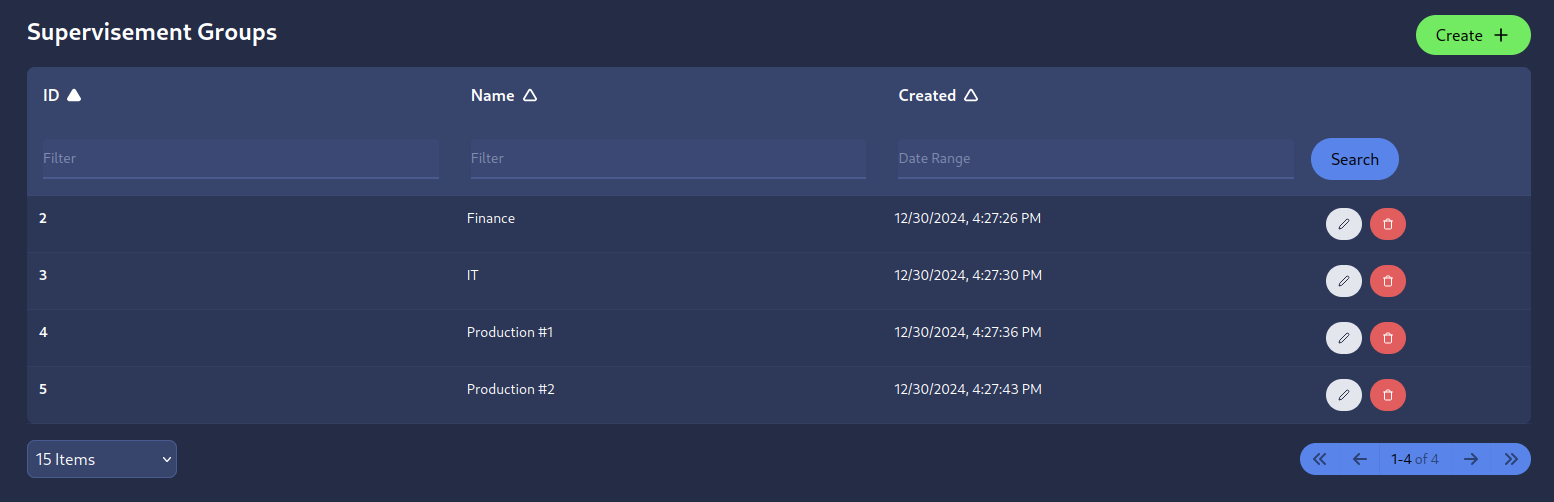
\includegraphics[width = 0.8\textwidth]{images/sup_groups.png}
  \caption{/admin/supervisement-groups oldal}
  \label{fig:sup_groups}
\end{figure}

\subsection{/admin/supervisement-groups/[id] oldal (BE) (10.25.)}

Befejeztem a tegnap elkezdett \inltxt{/admin/supervisement-groups} oldal implementálását. \\

Ezt követően létrehoztam a \inltxt{SupervisementGroupMemberships} adatbázis sémat (\ref{fig:sup_schema}.~ábra), amely a
dolgozók csoportokhoz rendelését valósítja meg.

\begin{figure}[ht]
  \centering
  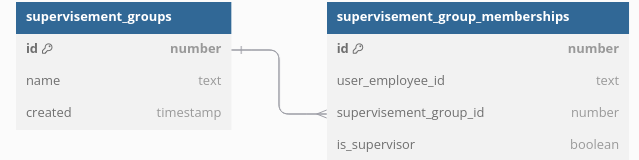
\includegraphics[width = 0.6\textwidth]{images/sm2.png}
  \caption{supervisement adatbázis séma}
  \label{fig:sup_schema}
\end{figure}

Utána a supervisement service-t egészítettem ki a következő függvényekkel:
\inltxt{addEmployeeToSupervisementGroup}, \inltxt{removeEmployeeFromSupervisementGroup},
\inltxt{editEmployeeIsSupervisor}, \inltxt{getEmployeesByGroupMembership}.\\

A fenti függvényekhez megírtam az \inltxt{/api} végpontokat, valamint elkezdtem írni a végpontokhoz
tartozó \inltxt{apiClient} függvényeket.


\subsection{/admin/supervisement-groups/[id] oldal (10.26.)}

Befejeztem a tegnap elkezdett \inltxt{apiClient} függvények implementálását, majd az
\inltxt{/admin/supervisement-groups/[id]} oldalt kezdtem el implementálni, amely két táblázatot
tartalmaz (\ref{fig:sup_edit}.~ábra). A bal oldali táblázat tartalmazza azokat a dolgozókat, akik még nincsenek hozzáadva a csoporthoz. Az
utolsó oszlopban található két gomb segítségével lehet hozzáadni őket (felettesként vagy
beosztottként). A jobb oldali táblázat pedig a csoporthoz már hozzáadott dolgozókat fogja tartalmazni.
tt az utolsó oszlopban lehetőség lesz a dolgozó eltávolítására a csoportból, valamint az
"előléptetésre", illetve a "lefokozására".


\begin{figure}[ht]
  \centering
  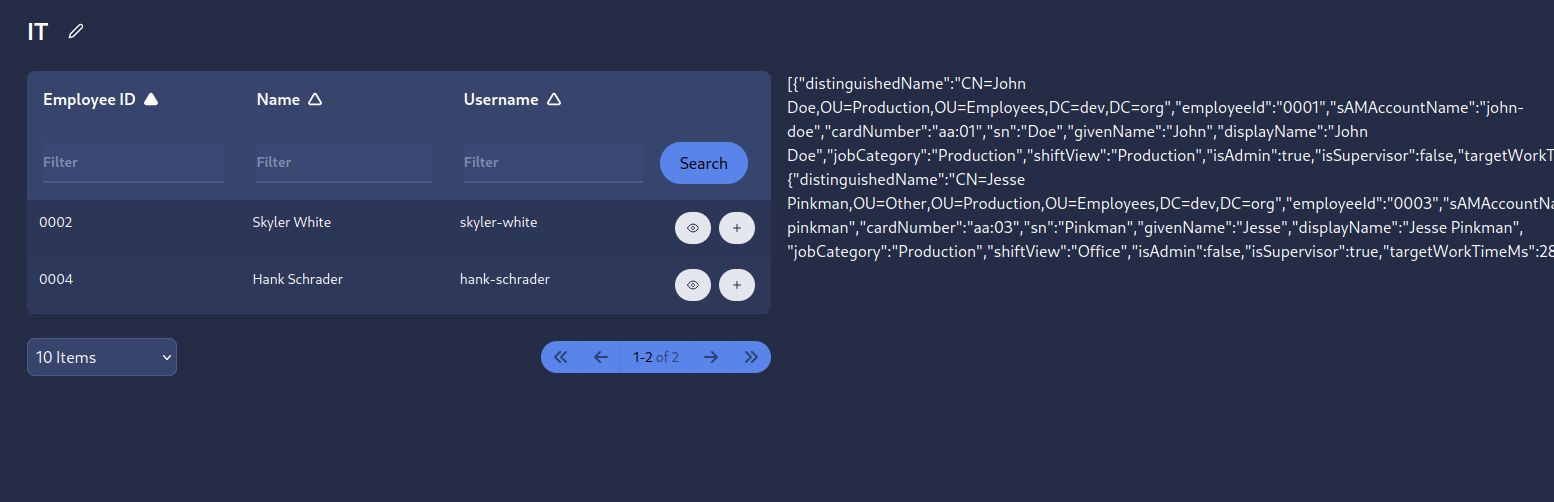
\includegraphics[width = 0.8\textwidth]{images/sup_edit.png}
  \caption{admin/supervisement-groups/[id] olda}
  \label{fig:sup_edit}
\end{figure}

\subsection{/admin/supervisement-groups/[id] oldal (2) (10.27.)}

Befejeztem az /admin/supervisement-groups/[id] oldal implementálását (\ref{fig:sup_edit_final}.~ábra).

\begin{figure}[ht]
  \centering
  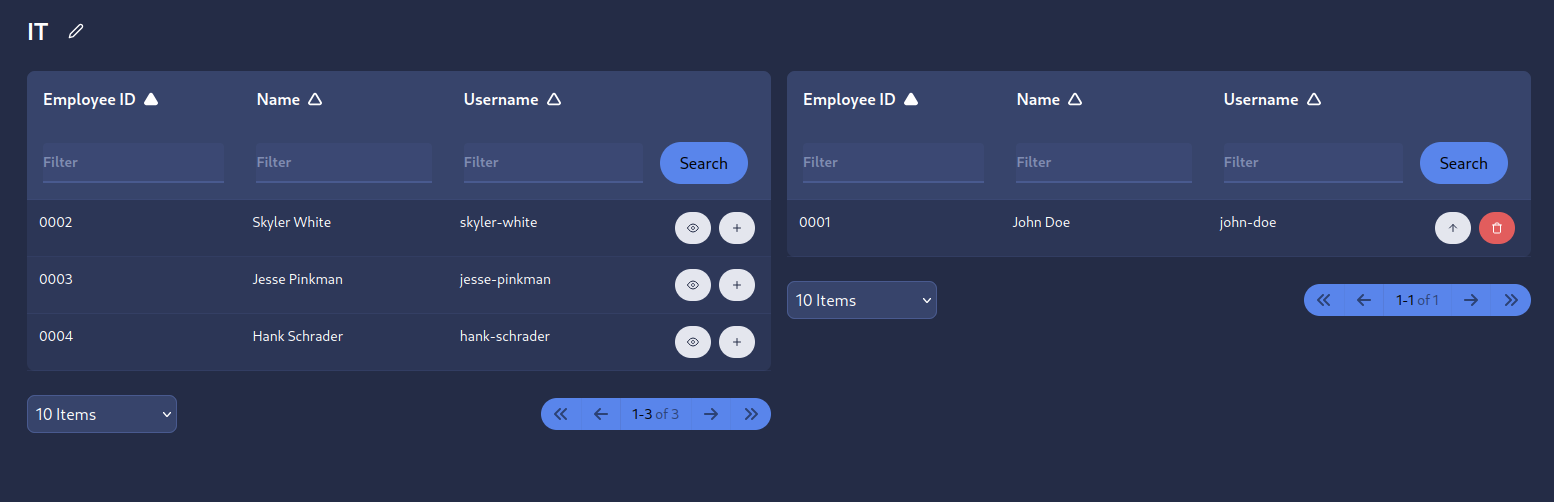
\includegraphics[width = 0.8\textwidth]{images/sup_edit_final.png}
  \caption{admin/supervisement-groups/[id] olda}
  \label{fig:sup_edit_final}
\end{figure}

\section{Hetedik Hét}

\subsection{isSupervisor függvények, dolgozó adatainak törlése funkció (10.30.)}

A supervisement service-t kiegészítettem az \inltxt{isSupervisor}, \inltxt{isSupervisorOfGroup} és
\inltxt{isSupervisorOfEmployee} függvényekkel, majd ezeket a függvényeket alkalmaztam, illetve
meghívtam minden szükséges helyen. \\

Ezt követően az /admin/employees oldalon elérhető "Dolgozó adatainak törlése" funkciót fejeztem
be, melyhez meg kellett írnom a
\inltxt{supervisementService.deleteEmployeeSupervisementRecords()}, a
\inltxt{cardUsageService.deleteEmployeeCardUsageRecords()} függvényeket, valamint a
szükséges \inltxt{/api} végpontokat.


\subsection{/supervisor/groups és /supervisor/groups/[id] oldalak (10.31.)}

A felettesek (supervisor) számára elérhető funkció implementálásán kezdtem el dolgozni. Ez a funkció
lehetővé teszi, hogy a dolgozó megtekintse a saját maga által felügyelt csoportokat. \\

Első körben a supervisement service-t egészítettem ki a
\inltxt{getPaginatedSupervisedGroupsOfUser()} és a \inltxt{getSupervisedUsersOfGroup()}
függvényekkel, majd az ezeknek megfelelő \inltxt{/api} végpontokat és az \inltxt{apiClient} függvényeket írtam
meg.\\

Ez után a \inltxt{/supervisor/groups}, valamint a \inltxt{/supervisor/groups/[id]} oldalakat
implementáltam (\ref{fig:groups_pages}.~ábra). A \inltxt{/supervisor/groups} oldalon a felettes megtekintheti a saját felügyelt
csoportjait. A jobb oldali oszlopban linkek mutatnak az egyes csoportok részletes oldalaira
(\inltxt{/supervisor/groups/[id]}). A részletes oldalon egy táblázat jelenik meg, amely az adott csoport
beosztott dolgozóit listázza. Itt a jobb szélső oszlopban a linkek az adott dolgozó munkaidő adatok,
valamint profil infó oldalára mutatnak.


\begin{figure}[ht]
    \centering
    \begin{subfigure}[b]{0.8\textwidth}
        \centering
        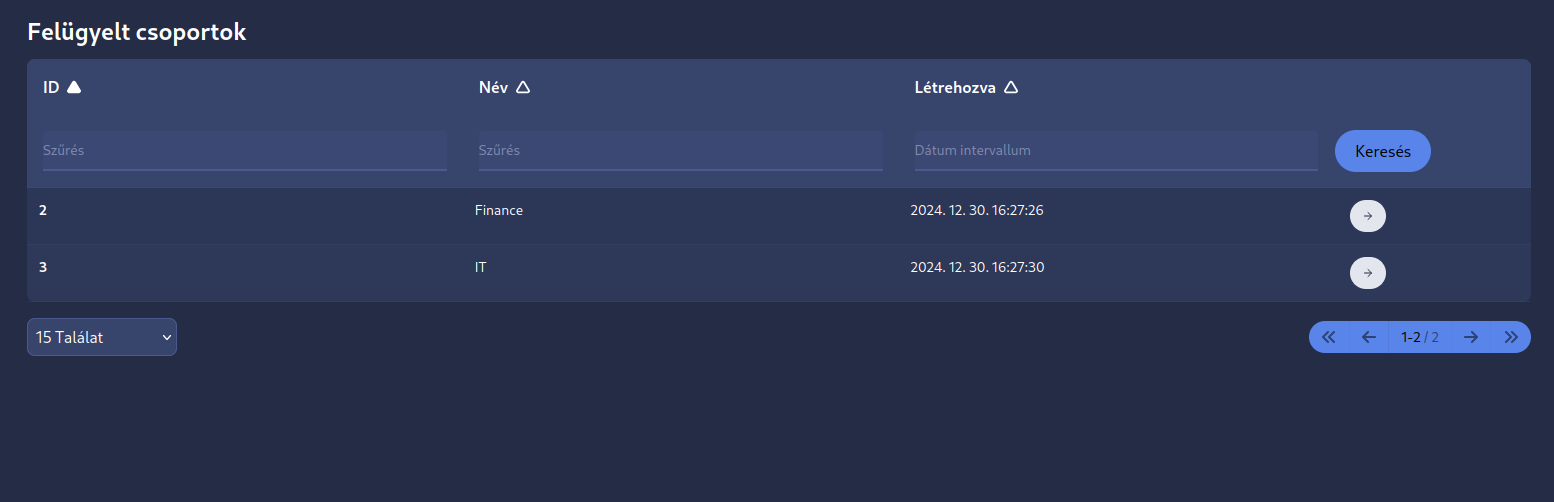
\includegraphics[width=\textwidth]{images/groups_page.png}
        \caption{/supervisor/groups oldal}
        \label{fig:groups_page}
    \end{subfigure}

    \vspace{1em} % Adjust vertical space between images

    \begin{subfigure}[b]{0.8\textwidth}
        \centering
        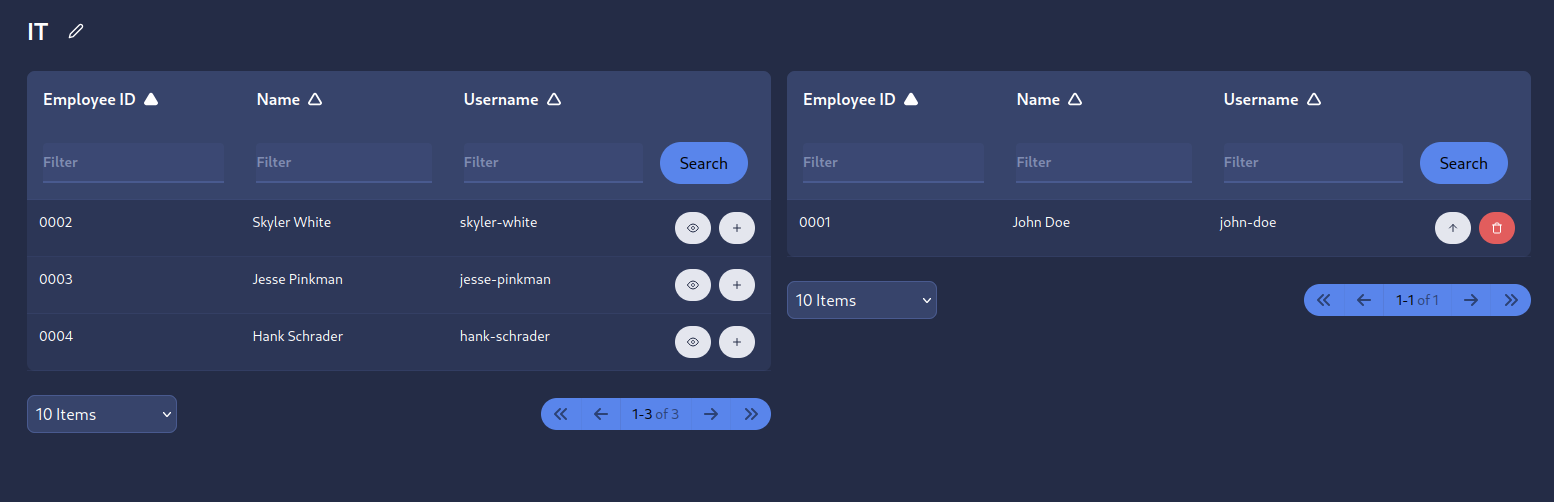
\includegraphics[width=\textwidth]{images/sup_edit_final.png}
        \caption{/supervisor/groups/[id] oldal}
        \label{fig:groups_id_table}
    \end{subfigure}

    \caption{/supervisor/groups és /supervisor/groups[id] oldalak}
    \label{fig:groups_pages}
\end{figure}

\subsection{Főoldal és hiba oldalak (11.01.)}

A mai napon a főoldalt, valamint a hiba oldalakat implementáltam (Ábra \ref{fig:home_page}. és \ref{fig:error_page}.).

\begin{figure}[ht]
  \centering
  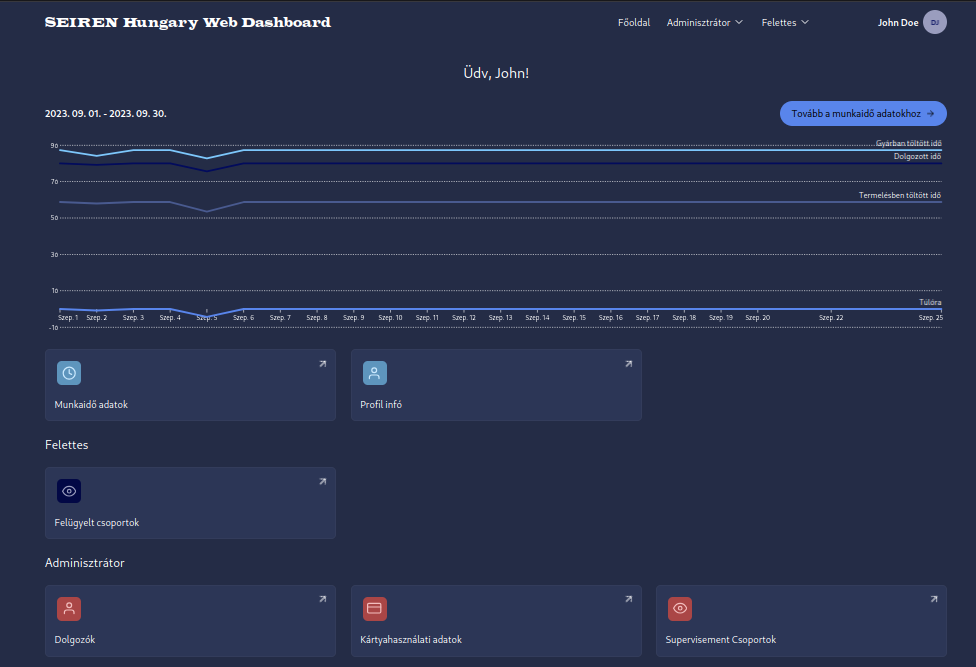
\includegraphics[width = 0.8\textwidth]{images/home_page.png}
  \caption{Főoldal}
  \label{fig:home_page}
\end{figure}

\begin{figure}[ht]
  \centering
  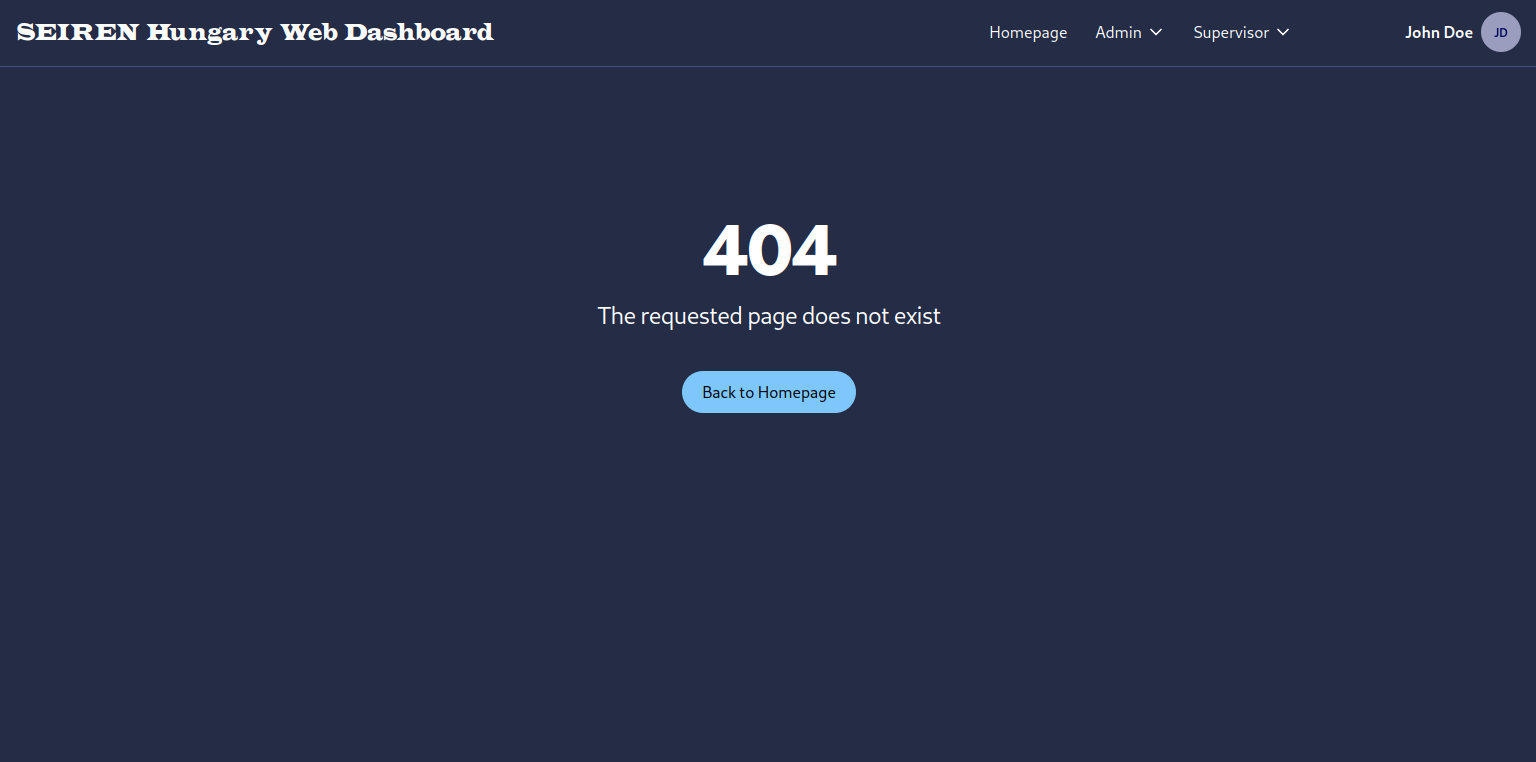
\includegraphics[width = 0.8\textwidth]{images/error_page.png}
  \caption{hiba oldal}
  \label{fig:error_page}
\end{figure}

\subsection{Dockerfile és docker-stack.yml (11.02.)}

Az alkalmazás telepítéséhez Docker-t szerettem volna használni, ezért először elkészítettem a
Dockerfile-t.\\

Első körben docker compose-t szerettem volna használni az alkalmazás, valamint az adatbázis
elindításához, azonban a docker compose-t eredetileg egy fejlesztői eszköznek szánták. Így esett a
választásom a docker stack-re, ami több - a későbbiekben potenciálisan használható - funkciót is
támogat (pl. secrets, rolling updates, rollbacks, orchestráció, stb.). A nap végére megírtam a docker-
stack.yml fájlt, amely három service-t tartalmaz: a dashboard alkalmazást, postgres adatbázist, caddy
reverse proxyt. Az egyik probléma, amibe ütköztem az az volt, hogy a docker stack nem támogatja a
környezeti változók fájlból való beolvasását. A végleges parancs a docker stack elindítására végül ez
lett:

\FloatBarrier
\begin{minted}[bgcolor=codebg, breaklines, breakanywhere, fontsize=\small]{bash}
env $(cat /srv/dashboard/deploy/.env | grep ^[A-Z] | xargs) docker stack deploy -c
/srv/dashboard/deploy/docker-stack.yml seiren-dashboard --with-registry-auth
--detach=true
\end{minted}

\subsection{GitHub Workflow (11.03.)}

Sajnos megfelelő mennyiségű teszt megírására nem volt elegendő időm. Ennek ellenére fontosnak
tartom, hogy legyen egy CI/CD pipeline, ami automatikusan lefuttatja a teszteket, style check-et, lint-
et, stb. Továbbá, az alkalmazás telepítésekor a docker image-et a docker engine egy privát Docker Hub
repository-ból tölti le, így a pipeline-nak az image buildelését és feltöltését is meg kell oldania. Ezt a
pipeline-t írtam meg a \inltxt{.github/workflows/pipeline.yaml} fájlban.

\section{Nyolcadik Hét}

\subsection{Szerver setup és dokumentáció (11.06.)}

Ma a szerver telepítését folytattam. Többek között létrehoztam a usereket, a könyvtárakat, azoknak
megfelelő jogosultságokat állítottam be, telepítettem a Docker-t, írtam egy szkriptet, ami letölti a
repository-t, majd kicsomagolja a deploy mappát, létrehoztam a docker secreteket, stb. Ezt követően
pedig elindítottam az alkalmazást, mely így már elérhető volt. Kérésre minden lépésemet
dokumentáltam.

\subsection{Riport fájlok szinkronizációja (11.07.)}

A Kantech (Windows) szerver és az alkalmazás szervere közötti fájlszinkronizációt oldottam meg. Több
lehetőség közül végül a unison nevű programra esett a választásom, amely ssh-n keresztül
szinkronizálja a riport mappákat a két szerver között. \\

Unison fájlok:

\FloatBarrier
\begin{minted}[bgcolor=codebg, breaklines, breakanywhere, fontsize=\small]{text}
# daily-report-sync.prf

root = C:\Users\Kantech-PC\Documents\EntraPass\Daily
root = ssh://reportuser@<host>//srv/reports/daily

sshargs = -i C:\\Users\\Kantech-PC\\.ssh\\id_ed25519
repeat = watch
auto = true
batch = true
confirmbigdel = false
confirmmerge = false

# emergency-report-sync.prf

root = C:\Users\Kantech-PC\Documents\EntraPass\Emergency
root = ssh://reportuser@<host>//srv/reports/emergency

sshargs = -i C:\\Users\\Kantech-PC\\.ssh\\id_ed25519
repeat = watch
auto = true
batch = true
confirmbigdel = false
confirmmerge = false
\end{minted}

Az a probléma lépett fel, hogy a unison ideiglenes (temp) fájlokkal dolgozik, így az alkalmazás azokat
a fájlokat is megpróbálta beolvasni. Egy reguláris kifejezéssel ki tudtam szűrni ezeket a fájlokat.\\

Ezúttal is minden lépésemet dokumentáltam.

\subsection{Két bug kijavítása (11.08.)}

Két bug kijavításán kezdtem el dolgozni. Az első mindössze annyi volt, hogy a "Profil gomb"-ban a
felhasználó nevének kezdőbetűi hard code-olva voltak, így ezt gyorsan kijavítottam.\\

A második, a munkaidők, vagyis a túlórák számolását érintő hiba volt. Ez egy komplexebb bug volt.
Nem is tudtam a nap végére kijavítani.

\subsection{Bug kijavítása, refaktorálás (11.09.)}

Először a tegnap megkezdett bug fixálását fejeztem be.\\

Ezt követően, mivel úgy tűnik, hogy az alkalmazás megfelelően működik, valamint új feature
megírására már nincs időm, a kódot refaktoráltam néhány helyen, így javítva kicsit a kódminőségen.

\subsection{Refaktorálás, issue-k írása (11.10.)}

Az utolsó napon, a tegnap megkezdett kód refaktorálást fejeztem be. Ezt követően a projekt során
felmerült ötleteket, kisebb bugokat GitHub issue-k formájában írtam le. Így, ha a későbbiekben más
hallgatók érkeznek a céghez, akkor könnyen folytatni tudják a projektet.

% \newpage
% % Blank page with page number
% \null
% \newpage

% Page with dotted signature lines at the bottom
% \newpage
% \vspace*{\fill} % Push content to the bottom
% \noindent
% \makebox[0.4\textwidth]{\dotfill} \hfill \makebox[0.4\textwidth]{\dotfill} \\[1.5ex]
% \makebox[0.4\textwidth][l]{\small Konzulens aláírása} \hfill \makebox[0.4\textwidth][l]{\small Hallgató aláírása} % Labels for the signature lines
% \vspace{1cm} % Add some spacing at the bottom
% \newpage


%% Page with two dotted signature lines and centered labels below them
% \newpage
% \vspace*{\fill} % Push content to the bottom
% \noindent
% \makebox[0.4\textwidth]{\dotfill} \hfill \makebox[0.4\textwidth]{\dotfill} \\[1.5ex] % Two dotted lines
% \makebox[0.4\textwidth]{\small \textit{Konzulens aláírása}} \hfill \makebox[0.4\textwidth]{\small \textit{Hallgató aláírása}} % Centered labels below the lines
% \vspace{1cm} % Add spacing from the bottom edge
% \newpage

% Page with single dotted signature line and centered label below it
% \newpage
% \vspace*{\fill} % Push content to the bottom
% \hspace*{\fill} % Push to the right
% \makebox[0.4\textwidth]{\dotfill} \\[1.5ex] % Dotted line
% \hspace*{\fill} % Push the text to the right
% \makebox[0.4\textwidth]{\small \textit{Hallgató aláírása}} % Centered text below the dotted line
% \vspace{1cm} % Add spacing from the bottom edge
% \newpage

\end{document}
